\chapter{Acquisition} \label{ch:3}

In recent work, a number of scholars (e.g., Bruner 1979, Snow 1979) have summarized the development of acquisition studies over the last two decades. In the mid-sixties, the field, which had previously been atheoretical and somewhat underdeveloped, came to be domi\-nated by a type of innatist theory. This theory, derived largely from generative grammar, and in particular from works such .as \citet{Chomsky1962}, held that the child acquired language through simple exposure to linguistic data, much of which was ``degenerate'' -i.e., consisted of st3n tence fragrnant11, mid-111;1ntrncr reformufo tiom, i:ind moi.ny types oJ performance error which would render natural speech a very unreliab mirror to mature native-speaker competence. Somehow the child had to sift the wheat from the chaff, and he could only do this, it wa claimed, if he had some kind of inbuilt Language Acquisition Device (LAD). A LAD would contain a set of linguistic universals, presumed to be innate and genetically transmitted. These universals would not\textsuperscript{1} however, precisely specify a particular potential language, as in the; theory described at the end of the last chapter; rather, they would de\-fine somewhat narrowly the limits on the forms which human language might take, thereby drastically reducing the number of hypotheses
that the child could make about the structure of his future native tongue and rendering it correspondingly easy for him to select the correct hypothesis.

Since it is well known that children, whatever else they may do, do not in fact instantly and unerringly make correct hypotheses about adult structures, but rather approximate to those structures by means of a fairly regular and well-defined series of stages, the innocent observer might have expected the next step to consist of an examination of the initial (and often incorrect) ``hypotheses'' made by the child, to determine why it was that that particular hypothesis, rather than any other, was originally selected. Further steps might have consisted of determining in what ways the child discovered the falsity of his original hypothesis and how he subsequently modified it (or selected an alternative) in order to approximate more closely to the linguistic models available to him.

Unfortunately, nothing of the kind was done. The founders of generative theory remained grandly aloof from the hare they had started, claiming that real-world acquisition processes were still too chaotic and ill understood to constitute a legitimate object of study and taking refuge in the ``idealization of instantaneity'' described in Chomsky and Halle (1968:Chapter 7). Workers in t1'e field were not simply left to their own devices; they were continually harassed by endless revisions of the theory. Doing acquisition work along Chom\-skyan lines became rather like playing a game which few minutes the umpires revise the rules.

Bearing this in mind-and bearing in mind too that workers in the field not only had no training in the analysis of variability and dynamic process generally but also had been given no reason even to think that such training might be necessary- it is not surprising that their results were somewhat unrevealing. In general, as shown, for example, in Brown and \citet{Hanlon1970}, \citet{Brown1973}, Bowerman ( 1973), etc., the predictions that generative theory seemed to make about acquisition were simply not borne out: young children did not
show conclusive evidence that they knew S -+ NP VP or other basic PS
%\originalpage{138}
rules; syntactic structures were not acquired in the order that was dictated by their relative complexity, and so on.

At the same time, and inspired at least in part by the meager results of generative-oriented work, many scholars began to question the assumptions on which this work was based. Was the input really degenerate? Was learning as rapid as had been claimed? Did it take place in the cognitive vacuum that at least seemed to be implied, if not actually asserted, in most generative writing? Upon examination, a number of these assumptions appeared to he partly or even wholly incorrect. Thus, there came about in the early seventies a very rapid and extreme swing of the pendulum, leading to an all but universal consensus among those working directly on acquisition which persists, with relatively minor variations, up to the present.

This consensus, while not ruling out entirely the possibility that some kinds of innate mechanisms may be involved in acquisition, systematically plays down and degrades the role of such mechanisms, often regarding them as constituting no more than a ``predisposition'' to acquire language, whatever that might mean (they never do say). The consensus holds, however, that prelinguistic communication and extralinguistic knowledge (acquired, nat urally, through experience) play crucially important roles in acquisition, hut that perhaps the most critical role of all is that of the interaction, paralinguistic as well as linguistic, which takes place between the child and the mother (or other caregiver). The mother, it is claimed, models language for the child, adapting her outputs to his linguistic level at every stage. Far from being degenerate, the data she provides are highly preadapted, highly contextualized, and patiently repeated. ``Mothers \textit{teach} their children to speak,'' \citet{Bruner1979} states. When all these factors are taken fully into account, the consensus claims, the need to posit an innate component in language acquisition shrinks to near zero or even disappears altogether.

Unfortunately, the whole position of this consensus is based on a fallacy-a fallacy that should be readily apparent to all readers of the two previous chapters. That fallacy is perhaps most concisely expressed
%\originalpage{39}
by Sow (197 :367) when she remarks that ``Chomsky's position regard.mg the, unimportance of the linguistic input was unproven, since \textit{all} \textit{c}\textit{.}\textit{htldren},\textit{.} m :UWition \textit{to} possessing an innate liuguistic ability, \textit{also} \textit{receive} \textit{a} \textit{smplifie,} \textit{wll-formed} \textit{and} \textit{redundant corpus``} (emphasis added). This 1s quite sunply untrue. The input that the first creole g.eneration in Hawaii received was over-simplified rather than simpli\-fied, and was as far from beiug well formed as anyone could imagine ;

and we can assume that in other areas where creoles formed the same state of affairs must have existed. Mother could not teach these children to speak, for the simple and inescapable reason that Mother herself di not know the language-the language didn't exist yet. But even so, without Mother, those children learned how to speak.

In adition to:his fallacy of fact, the Bruner-Snow position is base on a sunple log1cal fallacy. If we accept that in the vast majority of circumstances mothers do teach and children do learn, it by no means. follows that children learn BECAUSE mothers teach. It would be logically quite possible to argue that there is no connection whatso\-ever btween mothers' teaching and children's learning, any more than there is between ,children' walking and uncles' dragging them around the room by thetr fmgert1ps. If it could be shown that without well\-formed input from the mother the child could not learn to speak then we might indeed assume a causal connection. fn fact, we hav; sown the reverse: well-formed input from the mother cannot constitute eve a necessary condition for children to acquire language; for, otherwise, creoles could not exist.

But our argument, though logically correct, need not be pushed to its logical extreme. I am perfectly willing to accept that if mother did not teach her child English. that child might have a much harder tune learning it-even that the child might never acquire a perfected form of the language, but might significantly distort it in the direction of ,the. kind d pattern we reviewed in the last chapter. All I want to chum is that 1f we persist in believing that the child must have input m order to learn, we shall continue to misunderstand completely the way in which he does learn a developed, natural language. Just as
%\originalpage{140}
the child does not need mother in order to learn, so he could not learn even with a myriad of mothers if he did not have the genetic program that alone enables him to take advantage of her teaching.

In fact, the evidence we reviewed in the first two chapters of this book has simply never been taken into account in studies of child language acquisition. The vast majority of scholars in the f eld evince no awareness whatsoever of the existence, let alone the possible signi£cance, of pidgins and creoles; an honorable exception is Slobin (especially Slobin 1977). Unfort unately, the data available to Slobin at the time were by no means as ample as those given in the present volume; moreover, he makes the common mistake of supposing Tok Pisin to be paradigmatic of normal pidgin-creole development. Still, even limited access to pidgin-creole data is better for acquisitionists than none, and in consequence we shall find the work of Slobin and his associates illuminating on a number of points in the pages that
follow.

Meanwhile, in the absence of the insights provided by creolization, the current .paradigm has provided us with much information that we lacked before-on the nature of input to the child and of child\-caregiver interaction; on the acquisition of turn-taking, conversational routines, and the kind of social appropriateness summed up under
%\originalpage{141}
``acquisition strategy`` ``ha made us aware of some of the ways by which the child may possibly 'get into' the linguistic system. It has sl.iown us the importance of perceptual mechanisms for interpreting utterances, and how as adult speakers with full lingllistic competence we nevertheless rely on a number of short cuts to understanding . . . . The concept of language acquisition strategies has told us much -- except how the child acquires language.'' \citet{Bowerman1979} , who cites this passage with approval, further points out that while such strategies may enable children to understand utterances which still lie outside their developing grammars, those strategies do not and indeed cannot, in and of themselves, assign structural descriptions to rhese novel tterances. Yet children must achieve this kind of structural knowledge

1f they are subsequently to use such utterances themselves in a produc\-tive and creative way-understanding something is miles awav from manipulating that something freely and voluntarily. fn other ,words, strategies belong in the realm of performance, and the problem is, how do you get from performance to competence? Small wonder that so many supporters of the current consensus seek to downgtade, ignore,
or even abolish the competence-performance distinction. But real problems cannot be defmed away.

I propose, therefore, to review the literature on acquisition as
Hymes's concept of ``communicative competence H; on acquisition.

It concerns certain core syntactic and semantic structures, in particular
strategies'' based on contextualization, semantic and pragmatic clues to the function of novel structures, etc., etc.-and yet, as more and more thoughtful scholars are realizing, the gathering of this information has merely served to conceal the fact that the central question of acquisition, the question with which the early generativists did at least struggle, however unsuccessfully, is simply not being answered:

How can the child acquire syntactic and semantic patterns of great arbitrariness and complexity in such a way that they can be used creatively without making mistakes?

Cromer \{1976:353), for instance, observes that the concept of

some that we have had occasion to deal with in earlier chapters, to see whether what we know of the acquisition process supports or fails to support the hypotheses adva11ced at the end of the last chapter. To the extent that these hypotheses are supported, the general theory of a human language bioprogram will tend to be confirmed. To the

·extent that these hypotheses fail to be supported, doubts will be cast upon the theory, although the reader should perhaps be reminded that not even the most thorough refutation, in the arena of child language, would make the initial problem which led to the theory\-

the fact that creoles are learned without experience-miraculously ``'O

0

away. At worst, such refutation would merely drive us back to a
reconsideration of that problem.

%\originalpage{142}

But before commencing this review, three words of caution are in order: the first concerning the data; the second concerning the reviewer; the third concerning the theory.

From our point of view, the data suffers from two defects. First,
much of it has been presorted in ways that automatically diminish its utility. There are a variety of reasons for this, but I shall deal with oly one in detail, since it is fairly typical. A.round 1970, when acqu:si\-tionists were still concerned with proving (or disproving) generative predictions about acquisition, it appeared that one way of doing this would be to see whether features of a language were acquired in an order which conformed to some kind of hierarchy of grammatical complexity-simplest first, most complex later on. But In order to do this, it was necessary to determine exactly what one me;uit by ``acquisition of a feature.'' Children are such messy creatues; mste.ad of quietly going to bed one night without a feature, and waking ;'1th it, as the Chomskyan idealization of ``instantaneus acqu1S1tion'' suggests they should, they stubbornly insist on alternatmg p:esence and absence of that feature in appropriate contexts, not to mention absence and presence of that feature in inappropriate contexts, for periods of weeks, months, and occasionally even years.

Not only that, but the little beasts do not .even p\_roed. as
reason dictates they should, gradually and cumulatively drmmishmg inappropriate usages as they increase appropriate ones; on the contary, a graph of their appropriate productions zigzags up and down like a malaria victim's temperature chart, before finally leveling off at or near the 100 percent mark. The innocent observer might think that the
most interesting thing you could do in acquisition study would be . to figure out \textit{why} this happens, but as usual, he would e disappointed. Fashion and expediency dictate that order must be imposed on dts\-order: to determine the order of acquisition-a ``need'' dictated merely by current theory-\citet{Brown1973} established a .purely :1'bitrary ``.cri\-terion'' for acquisition, i.e., a 90 percent production rate m appropriate environments, maintained over three consecutive recording sessions. The reign of the criterion mere \{ reinforced what has always been
%\originalpage{143}
a trend in acquisition studies, and a deplorable one·\textsubscript{•}\textsubscript{ }to look to the o\textsubscript{0}-oal rather than the path, to ask ``What has the child acquired?'' rather than
``How has he acquired it?'' In consequence, masses of potentially valuable data, which would be required by any interesting acquisition theory, were simply flushed down the drain.l

In addition to deficiencies of this nature, we have to remember that all the data collected to date were collected for very different purposes than the present one. It is a general law applicable to all research that one tends to find what one is looking for, and not to fmd what one is not looking for. Hence, it would be unrealistic if we expected to find massive quantities of unambiguous evidence pointing toward the truth of our theory, which had yet somehow been missed by previous observers. The most that one can ever hope for from data collected under other assumptions and for other purposes than one's own are oblique hints, gaps that one's own hypotheses might fill, puzzles set aside that might begin to make sense in the context of a different framework. However, if one finds any of these at all, it is a reasonable assumption that a purposeful search of raw data sources would reveal much more-something comparable to the invisible eight-ninths of the iceberg.

With regard to the second word of caution, I can lay claim to no special expertise in the field of child language. In creoles, I have fourteen years' experience, most of them spent in direct contact with native creole speakers, so that I can speak in that field with some degree of confidence. In language acquisition, I can claim to be no
more than an assiduous reader of the literature, and in consequence, both. my knowledge and my understanding may be at fault sometimes. On the credit side, l can only offer complete uninvolvement m any of the controversies that have racked the field (for, as we shall see, my position, although innatist, is really no closer to the orthodox Chomskyan one than it is to the ``motherese'' school), and the freshness
of perspective that a novel viewpoint may on occasion bring. So be it: the facts will decide.

Finally, a word of caution about the theory. Straw-man versions
%\originalpage{144}
of innatist theories abound, and in particular, those which claim that to stress the function of an innate component in acquisition is auto\-matically equivalent to completely writing off all other modes of learning and all other aids to learning. In the present case, this par\-ticular straw man has even less substance than usual. The language bioprogram theory is, as we shall see in Chapter 4, an evolutionary theory, and the bioprogram itself is an adaptive evolutionary device. Now, it is the nature of such devices that they are facilitatory , not pre-emptive; that is to say , their whole adaptive function is lost if they force a species into a position where that species is dependent upon them and upon them alone, by inhibiting the action of other adaptive processes. In addition to whatever we may have in the way of innate language equipment, we also have a wide variety of learning strategies and problem-solving routines which are applicable to a range of situations far broader than language. It would be absurd to suppose that in the presence of data classified as ``linguistic,'' all these routines and strategies should simply switch off.

It would be equally absurd to suppose that they and the innate language component would be always and necessarily at war with one another. Sometimes their respective promptings may combine, some\-times they may point in opposite directions; which way is an empirical issue at anY given point. But their interaction must form the core of any complete description of language acquisition. If Ihave ignored
other resources in the present study , and have concentrated solely on the innate component, that is for strategic purposes only; besides, general cognitive processes have had far more than equal time in the last decade, and the turn of hardcore syntax and semantics has come around again. But Ibelieve that in order to acquire language-a feat which is, so far as we yet know, without parallel in the entire universe\-we need every ounce of help, particular or general, innate or acquired through experience, that we can get. To pit one kind against another simply demonstrates a failure to understand how complex language really is.\textsuperscript{2}
% {\textbackslash}
%\originalpage{45}
``.``'ith these preliminaries disposed of, we can begin our review. The eVJdence we shall consider will fall into two quite separate classes. One class will consist of the ``incorrect hypotheses'' which, in the course of language acquisition, children often make, yet which often seem t have o simpfo explanation either in the structure of the input th child receives or m any general theory of acquisition. The simi\-lanty between such ``hypotheses'' and the structures which actually em\_ege as part of the grammars of creole languages is often quite smk1:1g, and when I first contemplated writing this chapter, Ifelt certain that examples drawn from this class would constitute by far
the strongest evidence in favor of the bioprogram theory. After writing
the first draft of this chapter, however, I became much less certain, not so much because of the weakness of the original evidence-although there are. some phenomena, as Ishall show, which may allow alternative explanations-but because of the growing impression that a much subtler and less obvious class of evidence made on me.

As the ``icorret hypotheses'' suggested, there were many things m language .which children seemed to find quite difficult to learn, often spendmg years before they acquired full control over the struc. tuts concerned. n the other hand, there were certain other things wluch. seemed to .g e diem no trouble at all, which they learned very early m the acqmsmon process and/or without any of the ``mistakes'' which arose so frequently in other areas. On principle, one might suppose that these differences correlated with some kind of scale of relative difficulty, and yet it was extremely difficult to see exactlv what objective factors might constitute such a scale. Indeed, from commonsense linguistic viewpoint, some of the things that were easily and effortlessly acquired looked a lot more difficult to learn than some of the things that gave so much trouble.

But obviously, to talk about things being ``difficult'' or ``easy'' from an adult standpoint is totally irrelevant in an acquisition context. What is ``difficult'' or ``easy'' for the child is all that is of interest and one might therefore conclude that what seems ``difficult'' to u; might seem ``easy'' to the child, and vice versa. However, a moment's
%\originalpage{146}
thought should show that it was not so much the adult viewpoint as the use of the words ``easy'' and ``difficult'' themselves that was at fault in our original formulation.

Terms like ``easy'' and ``difficult'' imply an act of evaluation
which in t urn depends on the capacity to compare one task with another, which in turn depends on prior experience of tasks with differing levels of difficulty. Thus, when we acquire a second language, we can say that its derivational morphology, for example, is difficult to learn, while its relativization processes, say, are relatively easy. Such remarks are meaningful only because we already know a language and can measure features of the second language against those of the first. If we had not previously learned a language, we would have no standard of comparison; moreover, it is at least in part the nature of what we have already learned that determines whether what we are now about to learn will turn out easy or difficult for us.

Now, if we say that something is easy for a two-year-old to
learn, we cannot possibly mean any of this; all we can mean is that the child is somehow preadapted to learn that thing, rather than other things, or that in terms of the present theory , he is programmed to learn it. If, as we shall see is the case, the things that children learn early, effortlessly, and errorlessly turn out repeatedly to be key features of creole languages, which the children of first creole generations acquire in the absence of direct experience, we can then assume that such early, effortless, and errorless learning results, not from charac\-teristics of the input, or from the efforts of the mother-since the features involved are often too abstract to be known to any but the professional linguist-but rather from the functioning of the innate bioprogram which we have hypothesized.

I find evidence of this second class to be even more convincing
than that drawn from systematic error, and will accordingly begin by considering some examples of it. The first concerns the learning of the specific-nonspecific distinction (henceforth SNSD) by English\-speaking children. This distinction, as we saw in Chapters 1 and 2, is explicitly represented in all creole grammars by the opposition
% {\textbackslash}
% 
% ACQUISITION 147
between zero and realized determiners. It is expressed in English too, but much more obliquely, as we will see.

The most comprehensive study of the acquisition of English articles is that of Maratsos (1974, 1976), who confirmed by means of ingenious experiments the naturalistic observations of Brown ( 1973), i.e., that the article system is mastered at a very early age. Some of Maratsos' findings have been questioned in subsequent work (Warden 1976, Karmiloff-Smith 1979), but such criticisms relate only to the earliness with which the definite-nondefinite distinction is acquired. No one ·has challenged Maratsos' finding that the SNSD is handled virtually without error by three-year-olds, well ahead of the earliest date by which the child masters the definite-nondefinite distinction.

At first sight, this is an odd finding since the latter distinction is clearly marked in English, while the SNSD is not. In English, ``definite'' really means presumed known to the listener, whether by prior knowledge \textit{(} \textit{``the} man you met yesterday``), uniqueness in the universe \textit{(} \textit{``the} sun is setting``) , uniqueness in a given setting \textit{(} \textit{``the} battery is dead``-cars do not usually have more than one battery), or general knowledge that a named class exists \textit{(``the} dog is the friend of man``). ``Indefinite'' really means presumed unknown to the listener, whether by absence of prior knowledge (``a man you should meet is Mr. Blank``), nonexistence of a nameable referent (``Bill is looking for \textit{a} wife``), or nonexistence of any referent (``George couldn't see \textit{an} aardvark anywhere``). In other words, the two classes are systematically distinguished by the distribution of \textit{the} and \textit{a/an.}

Specific and nonspecific, however, are not systematically dis\-tinguished. Consider the following:

\ea\label{ex:1}
 If you're sick, you should see \textit{the} \textit{doctor} (NS).
\z

\ea\label{ex:2}
 Call \textit{the} \textit{doctor} who treated Marge (S).
\z

\ea\label{ex:3}
 \textit{The} \textit{doctor} may succeed where the priest fails (NS).
\z

\ea\label{ex:4}
 \textit{Dogs} are mammals (NS).
\z

\ea\label{ex:5}
 \textit{The} \textit{dog} is a mammal (NS).
\z

\ea\label{ex:6}
 \textit{A} \textit{dog} is a mammal (NS).
\z

%\originalpage{148}
\ea\label{ex:7}
\textit{A} \textit{dog} just bit me (S).
\z

\ea\label{ex:8}
 Mary can't stand to have \textit{a} \textit{dog} in the room (NS). 
\z

In fact·, the only way in which English distinguishes specifics from nonspecifics is in constructions with at least two articles. If a given referent is specific, it will receive \textit{a} on first mention and \textit{the} on second and subsequent mention:

\ea\label{ex:9}
 Bill bought \textit{a} \textit{cat} and \textit{a} \textit{dog,} but the children only like \textit{the} \textit{dog.}
\glt
\z

If a given referent is nonspecific, it will receive \textit{a} on first mention and on second and subsequent mention:

\ea\label{ex:10}
 Bill wanted to buy \textit{a} \textit{cat} and \textit{a} \textit{dog,} but he couldn't find \textit{a} \textit{dog} that he really liked.
\z



Maratsos constructed an ingenious set of stories which his child subjects were asked to complete. In some of the stories, reference was made to a specific entity; in others, to a nonspecific entity; in both cases, naturally, the entity was introduced into the story as \textit{a} \textit{N}\textit{P.} However, the completion task required the child to produce \textit{a} \textit{NP} just in case the entity was nonspecific, and \textit{the} \textit{NP} just in case the entity was specific, in accordance with the rule illustrated in /9/ and /10/ above (for full texts of the stories and a more complete description of the experiments, see Maratsos 1976).

The success rate in this experiment was almost 90 percent for three-vear-olds and over 90 percent for four-year-olds. In order to maintin these high rates, the children had to determine that out of some NPs identically marked, half had specific real-world referents and half had not. The stories were original and contained no contextual clues as to the status of the referents. How did the children succeed so often?

Maratsos himself was surprised and impressed by his subjects' capacities, and he discusses the implications of his experiments at
%\originalpage{149}
some length and with great insight. He notes that the high frequency
of articles in adult speech is often regarded as an adequate explanation
of the relative earliness and lack of error shown in the acquisition of articles. He points out, however, that ``although the frequency of [articles'] use may somehow serve to bring them to the child's atten\-tion and provide data for him, he must still select and attach to the articles just those abstract . differences in the circumstances of their use that correspond to the specific-nonspecific distinction. One clear requirement is that he have available some conceptual understanding of such matters as the difference between the notion of any member (or no member) of a class and that of a particular class member. This understanding must be sufficiently well articulated for the child to perceive just this difference in the circumstances of use of the definite and indefinite morphemes and construct the meaning of the terms accordingly'' \citep[453]{Maratsos1974}.

Let us try to reconstruct the process or processes by which the child might arrive at this perception. We will ignore the problems that arise from the child's original isolation and recognition of articles, although these are far from trivial (especially with \textit{a,} so frequently reduced to an unstressed schwa and so closely linked to its following NP that morpheme boundary perception becomes quite difficult), and deal solely with how, having recognized them, he determines their functions. If the conventional accounts are correct, the child can do this in only two ways-through linguistic context or through extralinguistic context.

The nature of the problems involved can be better understood if we compare the acquisition of articles with the acquisition of plural marking, which occurs at roughly the same age (a very few weeks later, according to Brown 1973). The plural morpheme marks a single, straightforward distinction-one/more than one-and it does so bi\-uniquely, that is to say, in a one-morpheme, one-meaning relationship: when the morpheme is present, one meaning is entailed; when it is absent, the other meaning is entailed. Articles are, from a purely formal viewpoint, much more complex than that. Three articles, \textit{the,} \textit{a,} and

%\originalpage{1}\zero, represent two distinctions-supposed-known-to-listener \textit{I} sup\-posed-unknown-to-listener and specific-referent \textit{I} no-specific-referent\-but without the biuniqueness that relates semantics to surface repre\-sentation in the c'ase of plurals. Instead, with regard to the second distinction only (the SNSD), there are two morphemes with one meaning (both \textit{a} and \textit{the} can have specific reference) and one mor\-pheme with two meanings \textit{(}\textit{a} can be both specific and nonspecific).

Let us suppose that the child can first factor out the distinction between \textit{o,} and \textit{the} (although in fact he cannot even rely on this aid; Warden [1976] and Karmiloff-Smith [1979] show that it will be several years before he is able to overcome this potential distraction). He then has to distinguish specific from nonspecific \textit{a. }One might think he could do this by distinguishing between linguistic environ\-ments. For instance, the scope of negation is often crucial in determin\-ing whether a given occurrence of \textit{a} \textit{NP} is specific or nonspecific: the difference between \textit{I} \textit{saw} \textit{a} \textit{dog} (S) and \textit{I} \textit{didn't} \textit{see} \textit{a} \textit{dog} (NS), for instance. So is the scope of desiderative verbs: the difference between \textit{I} \textit{want} \textit{a} \textit{dog} (NS) and \textit{I} \textit{have} \textit{a} \textit{dog} (S). Those who put their trust in extralinguistic context will, however, point out, quite correctly , that things like desiderative scope and negative scope are themselves ex\-tremely abstract relations, unlikely to be capturable by two-year-olds.

But in fact the problem is even tougher than we have suggested; there are many cases in which a mere tense switch marks the SNSD:

\ea\label{ex:11}
 When you see \textit{a} \textit{dog} (NS) , are you frightened? 
\z

\ea\label{ex:12}
 When you saw \textit{a} \textit{dog} (S), were you frightened? 
\z

Since the child's control of tense is, at the appropriate age, highly questionable at best, it is implausible to suppose that he could utilize such clues.\textsuperscript{3} Again, there are cases when desiderative scope alone is insufficient to mark the distinction:

\ea\label{ex:13}
 Your little sister wants \textit{a} \textit{dog-any} kind of dog (NS). 
\z

\ea\label{ex:14}
 Your little sister wants \textit{a} dog-and it's that one (S)! 
\z

% {\textbackslash}
% 
% ACQUISITION 151

In fact, the only reliable indicator of the SNSD is not a single article use, but a series of articles uses; an \textit{a-a }sequence, as in /10/ above, as opposed to an \textit{a-the} sequence, as in /9 / above.

However, as \citet[95]{Maratsos1976} again points out, it is at least highly questionable whether the child can take advantage of clues provided by sequences, especially when members of such sequences are not necessarily adjacent-as they are in /9 / and /10/-but may be separated by several sentences: ``It is easy to forget that the child, to the best of our present knowledge, does not have an extensive corpus of data at any one time with which to work. He probably cannot record numerous long stretches of conversation and all of the con\-textual information that accompanied them, as can an adult linguist investigating a novel language.``

We must therefore conclude that a child would be, at best, highly unlikely to derive the SNSD from analysis of purely linguistic context.

Yet is it any more likely that he could learn it from physical
experience or any other kind of extralinguistic source? As noted above, recent studies have concentrated heavily on the here-and-newness of speech aimed at children, and on the child's prelinguistic experiences in the world of objects. It is hard to see just how either of these could help with the SNSD. As \citet[94]{Maratsos1976} remarks, ``specific and nonspecific reference are connected in no clear way with external physical attributes or relations of perceived objects.'' For example, nonspecific reference is usually (although not always) made in the absence of any member of the referent class: \textit{we} \textit{don't} \textit{have} \textit{a} \textit{dogg}\textit{y}, \textit{Dad}\textit{d}\textit{y's} \textit{looki}\textit{n}\textit{g} \textit{for} \textit{a} \textit{doggy} \textit{for} \textit{you,} \textit{a} \textit{doggy} \textit{would} \textit{be} \textit{nice} \textit{to} \textit{play} \textit{with,} \textit{wouldn't} \textit{it?} and so on. But specific reference is made just as often in the absence of the referent : \textit{a} \textit{dog} \textit{bit} \textit{Jessie} \textit{yesterd} \textit{ay,} \textit{I} \textit{saw} \textit{a} \textit{dog} \textit{you'd} \textit{really} \textit{have} \textit{liked} \textit{in} \textit{town} \textit{toda}\textit{y}, and so on. How does the child determine that of the two absent sets of referents one is concrete while the other is only hypothetical? If he did not do so, he would score no better than chance on Maratsos' tests.

%\originalpage{152}

While it is true that many concepts are formed by the child prior to language learning, these are generally concepts which relate to physical objects which the child can see, touch, etc. Moreover, it is reasonably clear that such concepts ARE arrived at by interaction with experience rather than by merely processing language input. If the child only processed linguistic tokens of \textit{dog,} for example, he would pre\-sumably apply the term only to members of the appropriate species; whereas, as is well known, the initial meaning of \textit{dog,} for the child, is likely to be 'any four-legged mammal'. Thus, we know that the child reaches out ahead of linguistic experience, so to speak, in order
to derive ways of talking about the world.

But how could the child derive knowledge of purely abstract relationships from direct experience? A comparison with plural-marking acquisition is again very much to the point. Plural marking is directly associated with relations that the child is physically able to observe. He can see and feel at any given time whether he has one toy or several, whether he is allowed only one cookie or more than one ; the gramma\-tical marking of nouns correlates directly with manifest and obvious differences in his perceptual field. But the distinction between an actual member of a class (which more often than not is not physically present) and an imaginary representative of that same class is in no way one that · can be determined by the organs of perception, or inferred from any kind of direct experience. The SNSD involves comparisons, not between physical entities, but between purely mental representations; one can only marvel that a child, for whom the boundaries between . real and unreal are notoriously vague, should be able to make it at
all, by \textit{any} means.

Indeed, that he should even hypothesize such a distinction-a would, presumably, be claimed by those who believe in a hypothesis• forming, hypothesis-testing LAD-is highly implausible. Even abou possible functions of \textit{a} and \textit{the,} there are many possible hypothese that might be made. Since definites tend to be subjects while indefinite tend to be objects, one might hypothesize that \textit{the} marks agents and
% ACQUISITION 153
\textit{a} marks patients. Since \textit{the} often co-occurs with NPs that are physically present and \textit{a} with NPs that are physically absent one might hy\-pothesize that \textit{the }and \textit{a} mark poles of some kind of proximal-distal distinction. In fact, so far as we know, such hypotheses are never made. In any case, they would affect only \textit{a} and \textit{the; }with regard to \textit{a} alone, why on earth should the child even start by hypothesizing that there are really two kinds of \textit{a? }Moreover, since two-year-olds use few or no articles, and the SNSD is acquired by about the age of three, it would have to be just about the first hypothesis the child makes\-there would hardly be time to frame and discard any other. To say that the child invariably forms a correct hypothesis about the SNSD as his first hypothesis is simply an issue-dodging way of saying that he is programmed to make the SNSD.

Indeed, we can only conclude that the SNSD would be quite impossible to learn, by means of linguistic data, or of experience, or of any hypothesis-forming process, or of any feasible combination of these. For the child to make the SNSD as early and as successfully as he does, he would have to be somehow preprogrammed to make it.

This proposal is strongly supported by the creole data reviewed in Chapters 1 and 2. We saw there that the SNSD was made by the first creole generation in Hawaii (even though none of their HPE-speaking parents made it ) and that it is made consistently, and always by the same means, in all creole languages. If we assume a language bioprogram that includes the SNSD in its specifications, the prob]P.m of how the child acquires that distinction in English becomes a manageable nne. The child knows of the distinction in advance and is therefore looking put (at a purely subconscious level, of course) for surface features

.m the target language that will mark it. If no other feature is pre-programmed for NP, which is likely, then the fact that the SNSD
constitutes the child's first ``hypothesis'' is no longer bewildering, but
.M automatic consequence of the theory.
The skeptical reader may, however, ask: if creole children follow\-ing the bioprogram universally mark the SNSD by allotting zero marking to nonspecifics, how is it that children learning English, prior to
%\originalpage{1}
correctly interpreting the two \textit{as,} do not mark, or at least attempt to mark, nonspedfics with zero, as creole children do? The answer is that we do not know that they do not.

Earlier, I referred to deficiencies in the data due to excessive
concentration on the goals rather than the paths of acquisition. Here is a case in point. Even as conscientious and insightful a scholar as Maratsos confesses (1974:450) that ``only full noun phrases of the form article plus noun were counted; answers which included no article, such as \textit{boy, }were not counted in the analysis.'' Another careful inves\-tigator, \citet{Brown1973}, who allots some sixteen pages to a discussion of articles in early child speech, makes no reference to zero forms, and in what he claims is a ``full list of errors in definite and nondefmite reference for Adam, Eve and Sarah from Stages IV and V'' (1973: \tabref{tab:51}) includes only cases of \textit{a} where \textit{the} is indicated, and cases of \textit{the} where \textit{a} is indicated-no zeros at all. Yet from what Maratsos says, and from mere common sense, one knows there \textit{must} have been zeros; after all, the child has no articles at the two-word stage, and obviously does not acquire the surface forms overnight.

The present theory predicts that when a substantial body of early child language is properly examined, there will be found to be a significant skewing in article placement, such that a significantly higher percentage of articles will be assigned to specific-reference NP, while zero forms will persist in nonspecific environments longer than elsewhere. Such examination affords a simple and straightforward means of empirically testing the claims made about the innateness of the SNSD in this chapter.

We will now examine another distinction which is made even earlier and without , apparently, even a single reported case of error. This is the distinction between states and processes, including under the latter rubric verbs of experiencing as well as action verbs (hereafter referred to as the state-process distinction, or SPD). The SPD is di\-rectly involved in the acquisition of the English progressive marker
\textbf{\textit{-ing.}}

% {\textbackslash}

%\originalpage{155}

In general, the acquisition of novel morphology by the child is attended by cases of over-generalization, a number of which are dis\-cussed in \citet{Cazden1968}. Thus, the consistency in the final segments of possessive pronouns leads to production of the aberrant form \textit{*mines,} while plurals such as \textit{*sheeps,} \textit{*foots} (or \textit{*feets}\textit{),} \textit{*mouses,} etc., and past-tense forms such as \textit{*corned,} \textit{*goed} (or \textit{*wented}\textit{),} \textit{*buyed, }etc., occur in the speech of most, if not all, child learners of English.

The \textit{-i}\textit{n}\textit{g }form is acquired even earlier than the \textit{-ed} form (before
any of the other thirteen morphemes studied in Brown [1973], and as early as the second year in at least some cases). Also, just as there are verbs that do not take \textit{-ed,} there are verbs that do not take \textit{-ing} (with certain qualifications, see Sag 1973), such as \textit{lik} \textit{e,} \textit{want,} \textit{know,} \textit{see,} etc. These verbs are quite common in children's speech, probably as common as many of the irregular verbs to which children incor\-rectly attach \textit{-ed.} Yet, apparently, children never ever attach \textit{-ing} to stative verbs.

\citet{Kuczaj1978} has argued that the two cases are not really commensurate since with the past tense there are other ways of mark\-ing than \textit{-ed }(just as with plurals there are other ways of marking than

\textit{-}\textit{s}\textit{),} whereas in the case of \textit{-ing,} English has no alternative way of marking progressive aspect. This argument is somewhat disingenuous since zero can be a term in a subsystem, and it is hard to see what the difference would be between, on the one hand, adding \textit{-s} to \textit{sheep }to make \textit{sheeps} or \textit{-ed} to \textit{put} to make \textit{putted} , and, on the other hand, adding \textit{-ing} to \textit{like} to yield \textit{I} \textit{am} \textit{liking} \textit{you. }A more pertinent observa\-tion would be that verbs which do not take \textit{-ing,} as opposed to verbs which do not take \textit{-ed} or nouns which do not take \textit{-s,} constitute a natural semantic class; we shall return to this point in a moment.

In fact, Kuczaj undercuts his own argument by observing that children do indeed over-generalize \textit{-ing,} but not to stative verbs\-rather, to nonverbal items, as in /15/:

\ea\label{ex:15}
 Why is it weathering?\\
(presumably, 'Why is the weather so bad?')
\z



%\originalpage{156}

Note that, in fact, \textit{weather} is a plausible candidate for admission to the list of ``climatic'' verbs that yield expressions such as \textit{it} \textit{is} \textit{raining} \textit{/} \textit{snowing} \textit{/thundering, }etc. But all these verbs have in common the fact that they are nonstatives, as \textit{weather }would be also if it were a verb in the sense of /15/. The fact that children will generalize \textit{-ing} even to nouns IF AND ONLY IF SUCH NOUNS HAVE A PLAUSIBLE

NONSTATIVE READING makes their abstemiousness with respect to stative verbs even more significant.

Brown (1973:326ff) rightly regards it as remarkable that chil\-dren should be ``able to learn a concept like involuntary state before they [are] three years old,'' and explores several hypotheses which might account for such learning. In the case of one child, Eve, he was able to show that many nonstatives, as well as statives, were unmarked by \textit{-ing,} and that the unmarked nonstatives were precisely those which Eve's mother seldom used with progressive aspect ; on the other hand, the nonstatives which the mother did use frequently with \textit{-ing} were precisely those which appeared with \textit{-ing }in Eve's speech. However, a similar relationship did not hold for the other children in Brown's study; and as Brown himself pointed out, even if it had held, it would not have provided a solution. For anyone who claimed that children delayed applying \textit{-I}\textit{n}\textit{g} to a verb until they learned from experience that it was ``-ingable'' would then be forced to explain why a similar caution and restraint was not applied to other morphemes, like \textit{-ed }and \textit{-s,} where over-generalizations abounded.

Brown next considered the possibility that the SPD was learned from imperatives and transferred to progressives, since the verbs that will not take \textit{-ing} are just those that cannot be used in the imperative. Against this possibility, Brown argued that it would depend also on imperative usage being errorless; and it was simply impossible to tell whether this was the case since, especially in Stage I, children's impera\-tives are often formally indistinguishable from their declaratives \textit{(} \textit{want} \textit{cookie} looks like an imperative, but is probably no more than the child's version of 'I want a cookie').

A stronger argument against t)ie ``imperative transfer'' hypothesis,
%\originalpage{157}
not made by Brown, involves first recognizing that Brown's argument is in error; children could learn imperatives through trial and error and, having learned at last the list of verbs which could not be imperatives, simply apply that knowledge to the learning of \textit{-ing.} But trial-and-error learning of imperatives is more implausible than errorless learning of imperatives, and for the following reason: in trial-and-error learning, the child must correct himself simply through observing that others produce forms different from his (we know that overt correction of grammar, as opposed to content, is rare among parents). Thus, the child who says \textit{drinked} eventually becomes aware that others say \textit{drank} , and revises his grammar accordingly. If such things did not come to his attention, he would presumably go on saying \textit{d}\textit{rinked} indefinitely.

But negative evidence cannot function in this way. Let us sup\-pose that the child who said \textit{want} \textit{cookie} really was urging someone else to desire a cookie. Would the fact that he did NOT hear others saying

\textit{*want} \textit{some} \textit{chocolate} or \textit{*hate} \textit{naughty} \textit{bunny} deter him? It is hardly likely. I know of no facts which would indicate that a child needs positive reinforcement, as well as an absence of counterexamples, in order to maintain his current grammar. The child may be diverted from that ammar by the existence of contradictory forms to which he is obliged to pay attention; we can hardly expect him to pay atten\-tion to something that is NOT happening.

Moreover, on a purely pra,a,matic basis, trial-and-error learning of imperatives is unlikely. A child's early imperatives are all action\-oriented, aimed at getting people to pick him up or put him down, bring nice things to him and take nasty things away. It would be bizarre if he sought instead to influence the thought-processes and emotions of others by commanding them to want, need, know, etc. In fact, the likeliest possibility is that children do not acquire the SPD from imperatives, either errorlessly or by trial and error, because they them\-selves would only ever need nonstative imperatives for pragmatic reasons. They would not know whether statives could be used as imperatives because the opportunity for such use would simply not
%\originalpage{158}
have occurred-unless of course they were already programmed with the SPD, and thus ``knew'' that such uses were impossible, without requiring experience to prove it.

But whereas the use of imperative statives might seem bizarre, the use of progressive \textit{-ing} with statives would surely appear, to a child not programmed with the SPD, to be the most natural thing in the world. For \textit{-ing} is applied to verbs with present reference, and when a child wants or sees or likes something, it is right now that he does it.

\textit{*I wanting} \textit{teddy} \textit{(now}\textit{)} or \textit{*I} \textit{seeing} \textit{pussy} \textit{(now}\textit{)} would surely appear, to such a child, every bit as grammatical as \textit{I} \textit{playing} \textit{pee} \textit{k}\textit{aboo} \textit{(now}\textit{)} or \textit{I} \textit{sitting} \textit{potty} \textit{(}\textit{now)}\textit{.} Nobody could claim that the distinction emerged from experience, or from context; on the contrary, both experience and context would point in a contrary direction.

Finally, Brown considered the possibility that the distinction is innately known. However, he rejects this possibility because of what he claims are ``fatal difficulties.'' Since neither he nor other scholars who have discussed the issue (e.g., Kuczaj 1978, Fletcher 1979) have advanced any serious alternative to the innatist suggestion, we should examine Brown's ``difficulties``-bearing in mind that they arose out of a theory of innateness quite different from this one-and see whether they are really as ``fatal'' as he believes.

The first difficulty is that, according to Brown, children do not behave as innatist theory predicts with respect to categories other than state-process. If they came equipped with a full set of syntactic and/or semantic subcategories, ``they ought to attempt to order regular and irregular inflections in terms of one or another of the innate subcate\-gories. They should test the hypothesis that verbs that take \textit{-d }[sic] in the past are all transitives and the others intransitives or that those that take \textit{-d} are animate actions and the others not, or something of this kind'' (1973:328). Of course, this does not happen, and because it does not happen with distinctions other than the SPD, Brown con\-cludes that the SPD cannot be innate.

Now this argument makes sense only if you assume, first, that
% {\textbackslash}
% 
% ACQUISITION 159
children are born with all the subcategorization features of an \textit{Aspects} grammar in their heads (a view Brown specifically attributes to McNeil! [1966] ), and second, that children, like junior linguists, acquire gram\-mars by formulating and testing hypotheses. The present theory as\-sumes neither of these things. Thus, the fact that other distinctions were treated differently from the SPD could never constitute an argu\-ment against the innateness of the SPD, unless it could be shown that those other distinctions also formed part of the bioprogram. To do that, it would be necessary to show that those distinctions were for\-mally marked in creole languages. In creoles, animate actions are not formally distinguished from other types of action, and transitive verbs are not formally distinguished from intransitive verbs-quite the reverse, indeed, as we saw in the section on Passive Equivalents in Chapter 2, and as we shall see again later in this chapter. Thus, the child hy\-potheses Brown suggests would not make any kind of sense in light of the present theory, even if that theory supposed that children test hypotheses-which it does not.

Brown's second difficulty is that the SPD is ``a poor candidate
for innateness'' because it is ``very far from being universal in the world's languages.'' The problems foreign learners have with English progressives and a claim by \citet{Joos1964} that English is ``unique or almost unique'' in possessing the SPD are adduced as evidence for this \textbf{contention.}

Again, in the present theory, whether or not a given feature is common to all the world's languages is quite irrelevant. All previous universals theories have been static theories, which assume that lan\-guage is always and everywhere the same; if one accepts this, it follows that only features that occur in all languages can really qualify as can\-didates for innateness. But the present theory is a dynamic, evolu\-tionary theory which assumes that language had a starting point and a sequence of developments, which are recycled, in rather different ways, inhoth creole formation and child acquisition, as well as perhaps in certain types of linguistic change (consideration of which would take us beyond the scope of the present volume). What is innate is therefore
%\originalpage{1}
what was there at the beginning of the sequence, and thus there is not the slightest reason to suppose that innate features will automati\-cally persist and be found in the structure of all synchronic languages\-indeed, given the nature of dynamic processes, this would be an extremely unlikely result.

In other words, the SPD is presumed to be innate, not because of its universality, which may well be as low as Brown suggests, but because it plays a crucial role in creole grammars. There, statives are distinguished from nonstatives by the fact that the nonpunctual marker never attaches to the former ; but that is by no means the only signifi\-cant difference between the treatment of the two categories. The SPD causes a characteristic skewing of the creole TMA system, not explicitly treated in the present volume, but discussed at some length in Bicker\-ton (197 5 :Chapter 2). Briefly, there is a significant difference between creole and ludo-European systems which takes the following form. In the latter, the same morphological marking applies to both statives and nonstatives in any given tense; this seems so obvious that it is never even remarked on. In creoles, however, present-reference statives and present-reference 11onstatives carmot be marked in the same way, and the same applies to past-reference statives and nonstatives. The pattern for GC, which we may take as typical in this respect, is given in \tabref{tab:3}.1 below:
%\originalpage{161}
in creole grammar, his second objection to the innateness of the SPD is also deprived of its force.

However, Brown's claim that, if a distinction were genuinely
innate, it might be generalized to inappropriate environments (cited above in discussion of his fi'rst objection), is a reasonable one if it is made with respect to distinctions found in the bioprogram (as opposed to distinctions supposedly innate by the standards of other theories). An example which looks, from the data available so far, somewhat like
an inappropriate generalization of the SPD is found in data on the
acquisition of Turkish in Slobin and \citet{Aksu1980}.

Turkish has two morphemes used for marking pasHeference verbs: \textit{-dI} and \textit{-}\textit{m}\textit{i}\textit{s.} These are used in adult speech to mark direct experience (events personally observed by the speaker) and indirect experience (events reported to or inferred by the speaker), respectively. According to Slobin and Aksu, \textit{-dI} is usually acquired by age 1:9, and \textit{'mls} about three months later (i.e., about the same age as \textit{-i}\textit{n}\textit{g} is ac· quired). But ``at first the \textit{-dI} and \textit{-}\textit{m}\textit{i}\textit{s} inflections differentiate between dynamic and static events . . . . (C)lear differentiation of the two
forms [according to their adult meanings, D.B.] is not stabilized until.about 4:6.``4

The delay in acquisition is even more significant since most features of Turkish verb morphology are fully acquired at age 3:0. Although ``evidential'' tenses are found elsewhere (for example, in some
Present reference Past reference

Stative (/J bin

%%please move \begin{table} just above \begin{tabular
\begin{table}
\caption{1}
\label{tab:3}
\end{table}

Nonstative a

(/J

American Indian languages such as Hopi), they are completely un\-known in ``all creoles. From these two facts, we may conclude that the ditect/inditect experience distinction does not form part of the bio\-program, and .we may further hypothesize that non-bioprogram dis· tinctions that have emerged in natural languages are particularly vulner·

Stative-nonstative distinctions in GC

Thus, without a clear understanding of the SPD, the creole TMA system would be quite unworkable.

Since Brown believed that universality was the criterion for innateness, while the criterion for the bioprogram theory is emergence
% {\textbackslash}
able to reinterpretation in the conrse of the acquisition process. Such reinterpretation would naturally involve the assumption that the
surface markers of a non-bioprogram distinction were really marking a distinction . established in the bioprogram which is exactly what seems to be happening in the Turkish case. Certainly, any case of unusually delayed acquisition may tum out to be evidence as conclusive
%\originalpage{162}
of the workings of the bioprogram as are cases of early and errorless acquisition, once the mechanisms of interaction between bioprogram and target language are adequately understood.

We may therefore place the SPD alongside the SNSD as a second
semantic distinction (with important syntactic consequences) which is innately programmed. But consideration of the SPD naturally prompts the question: since among the most distinctive features of creoles is their distinctive TMA system, should it not be the case that this or a similar system emerges at some stage of acquisition, if indeed a uni\-versal genetic program generates such a system?

This question will serve to focus more sharply on the nature of bioprogram-target interaction, briefly mentioned two paragraphs above. In the present volume, emphasis is placed on the first member of the pair, for obvious reasons: until students of acquisition are convinced that a bioprogram is really operative, it is premature to talk too much about how such a bioprograrn might interact with other components of the acquisition process. But such emphasis can lead all too easily to a familiar straw man: the innate component which is supposed to roll like some irresistible juggernaut through the years of acquisition, sweeping all other influences aside. After the all too easy demolition of this travesty, the empiricist thinks he has disposed of innatism.

In fact, no innate program could or should behave in this way. From one viewpoint, the child is a biophysical organism evolving along the genetic lines laid down for its species, but from another and equally valid perspective, the child is a sociocultural organism growing up into membership of a particular human community. The pressures from the second side of being human must inevitably mold the impulses of the first-the more so since biophysical characteristics are typically more general and cultural characteristics more highly specified. Thus, from an early age-certainly from age two upward-we would expect that in a ``natural'' acquisition situation, as distinct from a pidgin\-creole one, the pattern of the bioprogram would be gradually shifted in the direction of the target-language pattern.

Such shifting must inevitabl\}'. affect the formation of a TMA
%\originalpage{163}
system. Since virtually all the relevant literature deals with acquisition of particular pieces of such systems, rather than with such systems as wholes, it is difficult to say at what age the child fully controls the TMA system of his mother tongue; but it is highly doubtful whether such control is achieved prior to age four, and likely that it may come considerably later than that. This means that the acquisition of TMA must spread over at least two years, two years during which the pres\-sure of the target grammar on the evolving bioprogram is steady and continuous. It would therefore be highly unrealistic to expect any child at any stage of acquisition to exhibit anything like a fully-developed creole TMA system. The most that we could expect would be that acquisition of the earlier features of TMA systems would be influ\-enced in rather oblique ways. However, if the results of such influence should prove mysterious to other theories of acquisition, yet follow logically from the present one, even such oblique evidence would be significant.

Accordingly, I shall re-examine two of the most influential papers on the acquisition of tense: Bronckart and \citet{Sinclair1973} and Antinucci and \citet{Miller1976}; and I shall show that some puzzling features of those studies become immediately clear once we assume that while the subjects of these studies appear to be merely learning French and Italian, respectively, the bioprogram decisively influences the progress of their acquisition.

One point must be made fu:st, however. With few exceptions, students of acquisition assume that when a child uses a past-tense form, he uses it because he fully understands, and deliberately intends \textit{t} mark, pastness of reference.\textsuperscript{5} True, it is often admitted (e.g., by Antinucci and Miller (1976]) that the child's concept of past may be restricted as compared with the adult's, and may extend only to past events. that leave. presently-observable consequences; but it is still assumed, without question, that where past marking appears, some sort of concept of past must be there too.

This by no means necessarily follows. All we can say is that
%\originalpage{164}
%\originalpage{165}
during the period in which past tense is being acquired, some past· reference verbs are tense.marked while some are not. There are several possible explanations of why this is so, none of which can be ruled
out a priori.

\begin{table}
GC

Past-marking rate

Punctual

38\%

Nonpunctual

12\%
\end{table}
 
The child may have acquired a full past rule but may
apply it unpredictably because of lapses of attention, phonological difficulties, etc. The child may have acquired a partial past rule which applies only to a subset of past.reference verbs. The child may have acquired a rule that has nothing at all to do with pastness or non\-pastness, but which just happens, coincidentally, to mark a certain percentage of past-tense verbs. Which of these explanations is the correct one can only be determined by empirical investigation in each individual case.

Since the study of variable data is much further advanced in decreolization than it is in acquisition, it should be instructive to look at another situation where variable past-morpheme insertion takes place. In creoles, past tense is not a category. But when creoles begin to decreolize, past-tense markers begin to be introduced, occurring sporadically just as they do in child acquisition.

At first, one might interpret such data just as similar child language data have been interpreted the speakers have an established past category but do not always mark it. However, analyses of de\-creolization in both Guyana and Hawaii (Bickerton 1975:142-61; 1977:36-51), with a data base of a thousand past-reference verbs in both cases, suggest quite a different picture.

On the assumption that speakers had a past category, one would have to conclude that decreolizing GC speakers randomly inserted past morphemes 27 percent of the time while decreolizing HCE speak\-ers did so 30 percent of the time. However, when all past-reference verbs were divided into two categories-those that referred to SINGLE, PUNCTUAL EVENTS, and those that referred to iterative or habitual events-insertion rates were shown to vary widely between the two categories, as shown in \tabref{tab:3}.2:



%%please move \begin{table} just above \begin{tabular
\begin{table}
HCE \textsubscript{53\% }\textsubscript{7\%}
Past versus punctual in decreolization
\caption{2}
\label{tab:3}
\end{table}


In other words, what was being marked in both sets of data was not really pastness, bnt rather punctuality.

The punctual-nonpunctual distinction (henceforth PNPD) is related to, yet distinct from, ·the SPD, and is of equal importance in creole grammar. Since both decreolization and acquisition involve the introduction of ``past'' marking where none was before, it should at least be worthwhile examining acquisitional data to see whether punctuality plays the same role in the second as it does in the f:trst. We should certainly do well to bear this possibility in mind while we reconsider previous findings on past-tense acquisition.

We may now turn to the first of the two papers cited above, Bronckart and \citet{Sinclair1973}. The authors' starting point was their informal observation that when children were asked to describe past events, their choice of tense often seemed to be influenced by the nature of the event : if the latter was one of some duration, like washing a car, they would tend to use \textit{il} \textit{lave} \textit{la} \textit{voiture} 'He washes/is washing the car', rather thanii\textit{a} \textit{lave} \textit{la} \textit{voiture }'He washed the car'; whereas if the
event was a punctual one, like kicking a ball, they would use \textit{il} \textit{a} \textit{pousse}%akzent?
\textit{la} \textit{balle} 'He kicked the ball', and seldom if ever substitute \textit{il pousse la}
\textit{balle} 'He kicks/is kicking the ball'.

Normally, the opposition between il \textit{lave} and il \textit{a} \textit{lave} is treated as a simple past-present opposition, but of course this is not the case. The ``present'' tense in French is in fact a nonpunctual aspect which does not extend into the past (unlike that of creoles); but, like a creole nonpunctual aspect, it embraces both iterative and durative events.

%\originalpage{1}

Similarly, the ``past'' is not a simple past in the sense of English simple past. English simple past is applicable to past-punct ual and past-iterative (but not always to past-0.urative) reference; French \textit{avoir} + participle is limited to past punct uals, while past iteratives and past duratives are rendered by the so-called ``imperfect'' form, e.g., \textit{il} \textit{lavait} rather
than il \textit{a} \textit{lave}.

In other words, when French children use different verb forms for different kinds of past events, they are doing exactly the same as creole speakers, who always mark nonpunctual pasts differently from
punctual pasts.

Bronckart and Sinclair confirmed and quantified their original observation by asking 74 children to describe (after the event) different types of actions which the investigators performed with the aid of a series of toys. Ages of the children ranged from under 3 to nearly 9. Eleven actions were performed. Of these, six were actions which had a clear goal or result (e.g., ``a car hits a marble which rolls very rapidly into a pocket``), while two were actions which had no perceptible goal
or result (e.g., ``a fish swims in the basin [circular movement J ``). The
three remaining ``actions,'' which consisted merely of cries of differing types or duration supposedly uttered by various toys, can be disregarded for our purposes.
of the six goal-0.irected actions, some were durative and others
were not. While the French \textit{passe} \textit{compose} was used more frequently for these six than for the two goalless actions, there was a significant
difference (p {\textless} .01) between durative and nondurative actions, the
former having a much higher probability of being marked with a nonpast (= nonpunctual) verb. The authors concluded that ``the dis· tinction between perfective and imperfective events seems to be of more importance than the temporal relation between action and the moment of enunciation. Imperfective actions are almost never ex\-pressed by past tenses, and for perfective actions the use of \textit{presents}
is the more frequent the greater the probability of taking into account the unaccomplished part of the action. This probability is partly determined by duration, frequence, [sic] , and maybe other objective features we have not investigated.``

%\originalpage{167}

In terms of the present study, Bronckart and Sinclair have dearly shown that the PNPD overrides the past-nonpast distinction until at least the age of six. However, the situation in French acquisi\-tion may be even more creole-like than the authors suggest.

First, they fail to mention the possibility that even when their subjects seem to be marking +past, they are in fuct marking +punctual. French-speaking children, like all other children, start out using the bare stem of the verb for every kind of reference, past or nonpast, punctual or nonpunctual, realis or irrealis. Then, at an age when devel\-opmental studies suggest that they have only the vaguest idea of past time, they encounter a form (the \textit{passe} \textit{compos}\textit{e}\textit{)} which has exclusively punctual reference. Note that, semantically, the categories of past and punctual overlap. While all pasts need not be punctuals, all punct uals must be pasts-if they were not, they would still be happening, and if they were still happening now, they would be nonpunctual by defini\-tion. Which is likelier-that they would interpret \textit{passe} \textit{compose} in terms of a distinction that they barely yet grasped (past-nonpast), or that they would interpret it in terms of a distinction which would be apparent to them from their own direct observation of actions and events (punctual-nonpunctual) ?

Second, there are a number of facts about the Bronckart and Sinclair data that the authors themselves either skim over or ignore altogether. In order to understand the significance of these facts, we shall have to re-examine their study rather minutely.

Let us begin by describing the six goal-oriented actions used in the study and then coding them in terms of type of action, duration, and iteration (where applicable). The actions (Bronckart and Sinclair's 1-6) are.as follows:

\ea\label{ex:16}
 A truck slowly pushes car toward a garage.
\glt
\z

\ea\label{ex:17}
 A car hits a marble which very rapidly rolls into a pocket.
\glt
\z

\ea\label{ex:18}
 The farmer junips over ten fences and reaches the farm.
\glt
\z

\ea\label{ex:19}
 The farmer's wife jumps in one big jump over ten fences and reaches the farm.
\glt
\z

%\originalpage{168} 

% ACQUISITION 169

The authors present (their \figref{fig:1}) a graph which shows the percentages of \textit{passe} \textit{compose} used to describe each of the different actions by members of five age groups, average ages of each group being as follows: 1, 3:7; 2, 4:7; 3, 5:6; 4, 6:6; 5, 7:8. Like all the acquisition charts I have ever seen , this one does not show a consistent\textsuperscript{6} and steadv rise from low to high percentages of correct forms; rather it shows he familiar fever-chart zigzags before coming to rest, at age
0
7 :8, with fairly uniform percentages of past marking across all action types.


In Bronckart and Sinclair's presentation, I think quite unintentionally, the amount of zigzagging is reduced by showing two different graphs for durative and nondurative events; thus, certain very interesting crossover phenomena, which are not accounted for in the authors'.conclusions, may very easily be overlooked.

In order to display these phenomena, I shall recast Bronckart
and Sinclair's data into the form given in \tabref{tab:3}.3 on the following page. In this table, the six actions, /16\{-/ 21/, are ranked for each of the first four age groups. Rank order is based on percentage of past\-tense assignment; thus, in each column the event at the head of the column is that which is most frequently assigued past marking, while the event at the foot of the column is that to which past marking is least frequently assigned. The nondurative items are circled in the
table for easier reference:

% The following table is not very nice :(
\begin{table}
	\begin{center}
		\begin{tabular}{cccccc}
			\multirow{2}{*}{Rank} & & \multicolumn{4}{c}{Age Group}\\
			\cmidrule{3-6}
			& & 3:7 & 4:7 & 5:6 & 6:6 \\
			\midrule
			1 & & P-1 & P-1 & J-1 & J-1\\
			\begin{tikzpicture}[baseline] \node [circle, radius=1.5] {2}; \end{tikzpicture} & & \begin{tikzpicture}[baseline] \node [circle, radius=1.5] {J-2}; \end{tikzpicture} & \begin{tikzpicture}[baseline] \node [circle, radius=1.5] {J-1}; \end{tikzpicture} & \begin{tikzpicture}[baseline] \node [circle, radius=1.5] {J-2}; \end{tikzpicture} & 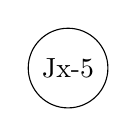
\begin{tikzpicture}[baseline] \node [circle, draw, radius=1.5] {Jx-5}; \end{tikzpicture}\\
			\begin{tikzpicture}[baseline] \node [circle, radius=1.5] {3}; \end{tikzpicture} & & \begin{tikzpicture}[baseline] \node [circle, radius=1.5] {J-1}; \end{tikzpicture} & 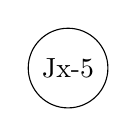
\begin{tikzpicture}[baseline] \node [circle, draw, radius=1.5] {Jx-5}; \end{tikzpicture} & 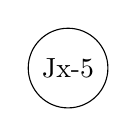
\begin{tikzpicture}[baseline] \node [circle, radius=1.5, draw] {Jx-5}; \end{tikzpicture} & \begin{tikzpicture}[baseline] \node [circle, radius=1.5] {J-2}; \end{tikzpicture}\\
			\begin{tikzpicture}[baseline] \node [circle, radius=1.5] {4}; \end{tikzpicture} & & 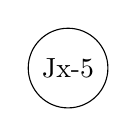
\begin{tikzpicture}[baseline] \node [circle, draw, radius=1.5] {Jx-5}; \end{tikzpicture} & \begin{tikzpicture}[baseline] \node [circle, radius=1.5] {J-2}; \end{tikzpicture} & \begin{tikzpicture}[baseline] \node [circle, radius=1.5] {P-1}; \end{tikzpicture} & 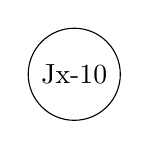
\begin{tikzpicture}[baseline] \node [circle, radius=1.5, draw] {Jx-10}; \end{tikzpicture}\\
			\begin{tikzpicture}[baseline] \node [circle, radius=1.5] {5}; \end{tikzpicture} & & 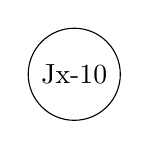
\begin{tikzpicture}[baseline] \node [circle, draw, radius=1.5] {Jx-10}; \end{tikzpicture} & 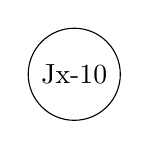
\begin{tikzpicture}[baseline] \node [draw, circle, radius=1.5] {Jx-10}; \end{tikzpicture} & 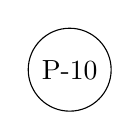
\begin{tikzpicture}[baseline] \node [circle, radius=1.5, draw] {P-10}; \end{tikzpicture} & \begin{tikzpicture}[baseline] \node [circle, radius=1.5] {P-1}; \end{tikzpicture}\\
			\begin{tikzpicture}[baseline] \node [circle, radius=1.5] {6}; \end{tikzpicture} & & 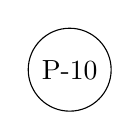
\begin{tikzpicture}[baseline] \node [circle, draw, radius=1.5] {P-10}; \end{tikzpicture} & 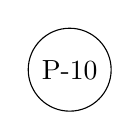
\begin{tikzpicture}[baseline] \node [draw, circle, radius=1.5] {P-10}; \end{tikzpicture} & 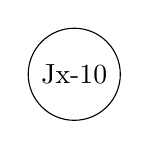
\begin{tikzpicture}[baseline] \node [circle, radius=1.5, draw] {Jx-10}; \end{tikzpicture} & 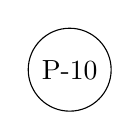
\begin{tikzpicture}[baseline] \node [circle, radius=1.5, draw] {P-10}; \end{tikzpicture}\\
			
			
		\end{tabular}
	\end{center}
	\caption{Rank orders for past-marking frequency}\label{tab:3}
\end{table}


%%please move \begin{table} just above \begin{tabular
\begin{table}
\caption{Rank orders for past-marking frequency. 3 presents a picture rather different from that which appears in Bronckart and Sinclair's tables and analyses. At the earliest age, actions seem to be ranked entirely on the basis of their duration, the shortest be.ing the most likely to be past-marked. The authors' \figref{fig:1} shows that the difference between the three highest ranks in the frrst column (i.e., those actions that have a duration of two seconds or less) is less than ten percentage points, while there is a gap of over twenty percentage points between the lowest of the nondurative actions and the highest of the durative actions (Jx-5).}
\label{tab:3}
\end{table}

However, this picture gradually and progressively changes, through the next three age groups: jumping actions irrespective of duration tend to rise in rank, while pushing actions sink to the bottom of the table. The final column shows durative and nondurative actions regularly interspersed, but the four jumping actions are now all placed higher than the two pushing actions. The authors' \figref{fig:1}shows that the stratification between jumping and pushing is quite sharp: while the
%\originalpage{170}
four jumping actions in the 6:6 column are grouped in a narrow range around the 90 percent past-insertion mark, the higher of the two push\-ing actions is separated from the lowest jumping action by a span of more than twenty percentage points.

Far from there being an overall rise in past marking of pushing actions, past-marking percentages for these show an absolute decline between ages 4:7 and 6:6, at the same time as past-marking percentages for jumping actions are rising fairly steadily. It stretches the imagina\-tion to suppose that children between these ages begin to perceive pushing actions as LESS past and jumping actions as MORE past; yet if we really believe that past tense is all that the children are ac\-quiring, we have no alternative but to believe in improbabilities such as this.

Bronckart and Sinclair note some of the fluctuations mentioned here, but attempt to account for only one of them , and that, perhaps, the least significant: the drop in rank for J-2 (their ``event 4``) be\-tween ages 3:7 and 4:7. The explanation they offer is that ``this action took objectively more time (2 sec.) than the others (1 sec.).'' By ``the others'' the authors mean, presumably, J-1 and P-1, but they are a little disingenuous here because they fail to note that the past-marking rate for J-2 ALSO FALLS BELOW THAT FOR Jx-Swhich takes more than twice as much time as J-2! Moreover, the rate for J-2 is only a point or two higher than that for Jx-10, which is five times longer! Relative length of time, therefore, cannot be the factor involved.

Let us see if we can really determine what underlies the phenomena illustrated in \tabref{tab:3}.3. From the first column, it would appear that children in the lowest age group do indeed discriminate between events on the basis of pure length. However, as they grow older, the criterion of durativity is replaced by another which is also related to the PNPD.

For the punctual-nonpunctual opposition must also be marked in the semantic features of individual verbs. That is to say, some verbs are inherently punctual, while others are inherently nonpunctual. lf you hit something for five minui;es, it must be that you hit it many
%\originalpage{171}
times; similarly, if you jump for five minutes, you must jump many times; both \textit{hit} and \textit{jump} express inherently punctual actions. But on the other hand, if you push something for five minutes you do not ncessaril push it more than once, and if something oils for five mmutes, It des not necessarily roll more than once; both \textit{push} and \textit{roll} express mherently nonpunctual actions (although of course a compound verb like \textit{roll} \textit{over} is inherently punctual).

. .fo other words, although the PNPD is crucial throughout the acqu1smon of past-tense marking, the way in which punctuality and nonpunctuality are interpreted changes as children mature. At f1rst, tey mere! register the relative length of events, and do not ·distinguish either the. mhe'.``6nt characteristics of different actions or any difference between iterative and durative events. Note how, in column 1 of

e grouped with P-10, the only truly durative event. Thus, their JUdgment of what is nonpunctual at age 3:7 accords with the common\-st ceole ju gment of what is nonpunctual: that is, a merger of the 1terat1ve (habitual) with the durative (progressive).

%%please move \begin{table} just above \begin{tabular
\begin{table}
\caption{3, the wo Jx events, which are sequences of punctual events,}
\label{tab:3}
\end{table}

However, as time goes by, the two Jx events are reinterpreted s squence of events, each one of which, considered individually , 1s bnef and mherently punctual. Thus, iteratives are removed from the nopunctual category (which now contains only duratives) and re\-asigned to the punctual category. This judgment- merging of iteratives with punctuals-corresponds to the minority creole pattern found in

Jamaican Creolr and perhaps a few others referred to under the heading of Dev1at10n E m Chapter 2 (p. 78J. It is certainly intriguing to speculate that at least some of the relatively few real differences in creoles c?uld result from their having been ``finalized,'' so to speak, at slightly
different age levels by the inventing generation-but of course we can only speculate at this stage.

What is of more immediate interest is the insight that we can denve, from the process described above, into the wav in which a bio\-program would evolve. Some scenarios for Chomsky innatism seem to suggest that every neonate already has a full \textit{Aspects} grammar curled
%\originalpage{1}
up in Broca's region. This literalistic reading of ``innate'' has no place in a bioprogram theory. A true bioprogram would grow, develop, and change just as the physical organism that houses it grows, develops, and changes. Increases in the child's cognitive abilities (which o course also form part of the bioprogram in its widest sense) would mteract with the linguistic component and progressively modify it.

For the French-speaking child, the shift in the nature of the
nonpunctual category would have the effect of moving ma.re events into the punctual category, thus making more events available for past marking. It would, in other words, help the child in his trai:sfer from predominantly punctual marking to predominantly past markmg\-although whether this result issues from the hand of a beneficent providence, or is merely an accidental bonus, it is far too early to tell.

The suggestion that children may have been marking punctality when they seemed to have been marking pastness may still see.m b12arre to some readers. Let us, therefore, see how well it stands up m hght of another well-known study of tense acquisition-that of Antinucci and
\citet{Miller1976}.
Antinucci and Miller found that the earliest tense form used by
their sample of Italian-speaking children was the past participle. At first this always agreed in number and gender with the sentential object, suggesting that the children regarded the participles as adjectives rather than verbs. Then, around age two, they dropped the agreement rule and began to use the participles in ways suggesting that they now perceived them as true past-tense verbs (the usual past tense in Italian consists of auxiliary plus participle, \textit{ho venuto }'I came', but the children almost always omitted the auxiliary).

However, the verbs which children used in this way appeared
to be somewhat restricted in number. The authors divided verbs into three classes: activity verbs (where the action has no end result) , stative verbs, and change-of-state verbs (such as \textit{close,} \textit{fall,} \textit{give,} et':'.) which describe actions as a result of which ``an object changes 1ts state.'' They found that with vry few exceptions, children's past
%\originalpage{173}
forms were found with verbs of the last class only, and they concluded that the child could only assign past tense to an action when some\-thing presently in his physical environment-a toy that had been broken, some milk that had been spilled-remained behind as a concrete result of that action.

Now, it happens to be the case that change-of-state verbs are all inherently punctual; the rare, apparent exceptions are often due to purely technological developments, as in \textit{the} \textit{abandoned} \textit{astronaut} \textit{fell} \textit{toward} \textit{the} \textit{planet} \textit{for} \textit{several} \textit{hours.} But even sentences like that can be
seen to be underlyingly punctual if we apply another test for inherent punctuality: the question, ``If you stop halfway through \textit{Vi}\textit{n}\textit{g,} have you \textit{Ved?``} Thus, if you stop halfway through closing, you have not closed, and if you stop halfway through giving, you have not given; similarly, if the abandoned astronaut stopped halfway through falling, he would not have fallen, although he migh t have lost altitude. But with activity verbs, which are inherently nonpunct ual, the converse applies: if you stop halfway through playing, you have played, if you stop half\-way through writing, you have written, and so on. If, as the Bronckart
and Sinclair study suggests; the more an action is regarded as punctual,
the more likely it is to be given past-tense marking, then the verbs in
ntinucci and Miller's change-of-state list may be given past marking bei:ause .they are. punctual, rather than for the reason the authors suggest:


It is true. that in the Bronckart and Sinclair study the first cri\-terion for the PNPD was raw duration, and that inherent characteristics
of verbs did not become dominant until an age long past that of the
Antinucd and Miller subjects. However, the Bronckart and Sinclair data are ·drawn from experiments, whereas the Antinucci and Miller data ate drawn from naturalistic observation; moreover, Bronckart and inclair do not include any change-of-state verbs in their study. The .two studies are therefore not comparable at the fine-grained level 6f,.``Just how do children interpret punct uality at age X?``; they do, ho{\textbackslash}Ver, seem to be in agreement that some kind of PNPD is involved.
There are other clues in Antinucci and Miller's study which
%\originalpage{174}
suggest that a punct ual analysis may account for the facts better than a change-of-state one. Early in their third year, Italian children generally acquire a second Italian past tense, the imperfect. This is used with activity verbs, but is not extended to change-of-state verbs, which continue to be past-marked with participial forms (with or without auxiliary):

\ea\label{ex:22}
 (Antinucci and Miller's 82)\\
  Mamma \textit{e} \textit{andato} (participial) al parco e io \textit{stavo} (imperfect) \textbf{a} \textbf{casa}\\
\glt'Mommy \textit{went} to the park and I \textit{stayed} home'
\z







\ea\label{ex:23}
 (Antinucci and Miller's 90)\\
  Li \textit{ha} \textit{messi }(participial) nel saco e dopo gli altri bambini \textit{piangevano }(imperfect) \\ 
\glt 'He \textit{put} them in a sack and then the other children \textit{cried'}
\z





In other words, imperfects and participials are in complementary distribution, the first being used for punctual verbs, the second for nonpunctual ones. Note that this does not reflect anything in Italian grammar; all Italian verbs, whether punctual or nonpunctual, activity or change-of-state verbs, have both perfective and imperfective past \textbf{tenses. ,}

Antinucci and Miller's explanation for this state of affairs is far from satisfactory. They note that the imperfect appears first during story-telling, and suggest that the child uses it to distinguish ``pretend'' from real events. But if this were really the case, we would expect use of the imperfect to be extended to all types of verbs, including change\-of-state verbs; for surely change-of-state (or punct ual) verbs can be used to describe imaginary events as easily as activity (or nonpunctual) verbs. Moreover, in the examples that Antinucci and Miller themselves cite, such as /22/ and /23/ above, the events of \textit{staying }and \textit{crying,} rendered by the imperfect, are no more (or less) ``pretend'' events than the events of \textit{going} and \textit{putting, }which are rendered by the participial form. ,

%\originalpage{175}

It is therefore highly possible that the connection observed by the athors bet``'.'ee ``pretend'' evnts and the imperfect is merely a part1 .and comc1den tal one. It 1s hard to tell, since they present no stat1st1cal data that would serve to quantify the distribution of participial and imperfective forms in realis and irrealis contexts. And if their hypothesis is falsified even by the few sentences they themselves choose \textit{to} cite, and if both tenses are past-reference in adult speech, then there is nothing but the PNPD to prevent children from general\-izing the more regular, imperfect form to change-of-state verbs just as English children generalize \textit{-ed} to irregular pasts. '

Inded, hw is it that English children generalize in this way when Italian children do not? If everyone has the same bioprogram, how com.e everyone doesn't learn the same way? Let us explore this problem 1Il some depth, for by so doing we will not only answer these and other questions, but we will also better understand how the same
bioprogram can yield superficially different results when it interacts with two languages that differ in structure.

First, let us dispose of a possible objection. It might be argued tat the two processes- Irian-speaking children learning first parti\-ciples, then llnperfects; English-speaking children learning first irregular, then regular pasts-are not really commensurate. So they are not, from an adult point of view. But the child does not have an adult point of view, and for the child they must be completely commen\-surate. The adult knows that Italian has two tense forms with different meanings, whereas English has only a single form, expressed in diverse ways. But there is no way a child could know this unless he were born with a comparative grammar of Inda-European in his head, as well as \textit{Aspects. }Remember, the children we are talking about are under three. Not only can they not have the slightest idea what the mat ure tense system of their languages will eventually look like, but even on the most favorable accounts, they can have only the vaguest notion of
what past means, and by some accounts, they can have no notion at all.

%\originalpage{176}

What must really happen is something like the following. Around age two, the child who happens to be learning Italian becomes aware of a set of rather irregular forms, which are past-reference forms in adult grammar (the Italian participles), whereas the child who happens to be learning English also becomes aware of a set of rather irregular forms, which are also past-reference forms in adult speech (the English ``strong'' past tenses). Shortly afterward, the child learning Italian encounters a set of quite regular forms, once again past-reference forms in adult speech (the Italian imperfective), while, around the same time, the child learning English also encounters a set of regular forms that are past-reference forms in adult speech (the English ``weak'' past tenses).

Up until this point, the experiences of the two children have been , from their point of view, identical. I defy anyone to explain how those experiences could be differently interpreted by the two children-except in a single respect, which we shall deal with shortly. From the child's point of view, in both cases he has begun by finding some irregular fors that mean past (from the traditional perspective) or punctual (from the perspective of this volume), and he has gone on to find some regular forms that also mean past (from the traditional perspective).

But now, the Italian learner and the English learner part com\-pany. The Italian learner keeps the two sets of forms, the regular and the irregular, completely separate, applying one set to one class of verbs and the other to another. The English learner, on the contrary, proceeds to generalize the regular set to the irregular set, applying ``weak'' tense endings to ``strong'' verbs in defiance of adult grammar rules. Why ? Why doesn't the Italian learner make a similar generaliza\-tion? Or, to put it differently, why doesn't the English learner make the same kind of distinction as the Italian learner, maintaining the irregular forms (like \textit{came,} \textit{went,} \textit{bought,} \textit{sold,} \textit{gave,} \textit{broke-all} good changes-ofstate, note) for punctual verbs, and saving the \textit{-ed} affix for activity verbs?

To understand the answer, we have to get used to looking at the
% {\textbackslash}
%\originalpage{177}
acquisition process in a way it has not been looked at hitherto-even though e.verything w.e know about language points to that way as the mst logical and fr1tful. Als, the ``order of acquisition'' gambit set child language studies back fifteen years by concentrating exclusively on the acquisition of isolated features. Small wonder if, as we have seen, the sterility of this approach sent acquisitionists gamboling off across the meadows of pragmatics, cognition, ``motherese,'' etc., which were not much more irrelevant to the central problem of syntax acquisition, but a good ?eal less dull. For what both groups forgot was that lauage IS a tight system composed of even tighter subsystems. Children do not learn individual morphemes in isolation from
one another; they build up subsystems and at the same time integrate those subsystems into an overall system.

The situation was not helped any by the primitive state of the art in TMA studies, in spite of (I would prefer to say, because of) wo'.k in the field from \citet{Reichenbach1947} to \citet{Comrie1976} and Wo1setschlaeger (1977). We shall return to this issue in Chapter 4; for. the .moment, suffice it to say that an approach like Comrie's,
which tries to extract some kind of Platonic core meaning from terms like ``perfective'' and ``imperfective,'' totally ignores the fact that the units of grammatical subsystems cannot be defined independently of those systems-that, in consequence, what ``perfective'' and ``imperfective'' mean, in any subsystem where such labels are applicable,
IS entirely determmed by how many other units that subsystem has and what the other units mean.

Once this viewpoint is established, we can proceed to look at the acquisition of TMA systems AS SYSTEMS, bearing in mind all the while the injunction of the bioprogram; ``Make sure that punctuals and nonpuncts are adequately differentiated.'' We may then represent the acquisition process for English and Italian learners as in Figure
3.1% on the following page:

%\originalpage{1}

\begin{figure}
Time line (very approx.)

\textsubscript{1}\textsubscript{:6 }\textsubscript{-}---------------2:6

-ing (NP)
 
\end{figure}

that the scope of this ``present tense'' differs in English and Italian; in English it includes habitual and iterative reference only, whereas in Italian it includes progressive and durative reference also. The child,

·needless to say, cannot foresee these facts, but they exert a profound influence on the acquisition process, as the following paragraphs will show.


\begin{figure}
English learner

base{\textless}

base

{\textless}irr. past (P)

base

reg. past

base
\end{figure}


The question of what determines the order in which new forms
are acquired is too complex to be explored fully here.\textsuperscript{6} However, it seems likely that the difference between Italian and English present tenses determines the first addition to the system. English has a dis\-tinct (and frequent) form for present progressives; Italian has not. Therefore, the first new term that English learners add is a nonpunctual one. But since there is no similar form in Italian, the first new form that Italian learners add is a past form-the participle-which they interpret as a punctual one.

\begin{figure}

Italian learner

base {\textless}P``'part. (P)

base

1'1gure 3.1 .

Comparative TMA acquisition (Italian versus Enghsh)
\end{figure}



The second new form acquired by English learners is the ir\-
regular past, which they interpret as marking punctuality. They are therefore now able to mark both sides of the PNPD. But shortly after\-ward they become aware of a third form-regular past \textit{-ed.} Since they already have markers for punctual and nonpunctual, they cannot ac\-commodate this .new form by assigning to it its own semantic scope; they therefore assume they were wrong in choosing irregular past as a punctual marker, and proceed to extend \textit{-ed} to those past punc\-tuals which had previously been allotted irregular forms.

However, the second new form acquired by Italian learners
is the imperfect. This, like the past participle, is used for past reference by adults, and if Italian learners were really using participles to mark past reference, they would surely generalize the imperfect form to

%move footnote
Both English and Italian learners begin with a single undiffe
entiated base form which at . first has to cover all intende.d forms \textsubscript{TMA}\textsubscript{ }\textsubscript{r}\textsubscript{e}\textsubscript{£}\textsubscript{erence}\textsubscript{ }\textsubscript{·}·(\textsubscript{m}· f\textsubscript{a}\textsubscript{c}t\textsubscript{'}\textsubscript{ }the Italian base form is reall\textsubscript{.}y a s\textsubscript{.}eries of\textsubscript{.}\textsubscript{ }for differentiated for person, but this and similar details will be ignored
here for the sake of clarity of presentation). As ne:V- .forms are. add
verbs of all types, just as English learners generalize -ed-Jor, as noted
above (p. 176), the Italian participial/imperfect opposition and the
English irregular/regular past opposition must look formally identical to the child learner. The reason why they do not do this can stem only from the unique difference between the situations of the two the
semantic
scope of this base form contracts until it evolves into t
sets of learners: English learners have already marked both sides of
adult, so-called ``present tense'' in both languages. Note, however
%\originalpage{180}
the PNPD, while Italian learners have marked only one side. For them, nonpunctuals are yet to be marked, so instead of generalizing the imperfect, they seize on it as their nonpunctual marker and keep it carefully separate from their marker of punctuality , the participial form.

Note that without the bioprogram the differences in behavior between Italian and English learners are quite inexplicable. In virtually identical circumstances, the English learner over-generalizes, while the Italian learner under-generalizes. However, once we see that English and Italian learners are equipped with an identical program, but still satisfying the requirements of that program in a different order-an order determined by the interaction of the bioprogram with two different languages-such differences are not merely explicable, but follow inevitably from the theory presented here.

Now we can better understand what the child of a first creole generation does. When that child is around 18 to 21 months old, his TMA ``system'' and the TMA ``system'' of his parents' pidgin exactly coincide; both consist of the ``universal base'' shown at the left-hand side of \figref{fig:3}.1. The only difference between the child's trying to learn a pidgin and the child's trying to learn French or Italian is that the latter will be offered a variety of verb forms which he can then interpret according to the specifications of his bioprogram, while the former will not be offered anything new in the way of forms. The creole child therefore decides to mark the nonpunctual side of the opposition.

Two questions may be asked here: why does the creole child decide, apparently without exception, to mark nonpunctuals rather than punctuals, and why does he not mark both terms of the opposi\-tion, as I have claimed that both English and Italian children do?

I think that nonpunctuals rather than punctuals are marked because, from a pragmatic viewpoint, nonpunctuals represent the marked case in a Jakobsonian sense: in the real world, more actions are punctual than nonpunctual; punctual actions constitute the back%
%\originalpage{81}
ground against which nonpunctual actions stand out. Regarding the second question, we should rather ask, why do noncreole children mark both terms? The answer to that clearly is because noncreole children receive, if anything, too great a variety of forms-greater, certainly, than any two-year-old can incorporate into a coherent system. The child feels obliged to assign some kind of significance to terms with which he is constantly bombarded, so he assumes that in the language confronting him both sides of the PNPD are formally marked.

But, of course, both sides of an opposition do not have to be formally marked-it serves to distinguish them if you formally mark one term and zero-mark the other. Considerations of parsimony alone would indicate such a choice, if the opportunity presents itself (and for the creole child, it does). It is quite enough trouble for the creole child
to select, from the pidgin, one content-word (like HPE locative \textit{stei)}
to mark one term of the opposition, without having to search out another to mark the other. In both cases, albeit by differen t means, the demands of the bioprogram are satisfied.

I have little doubt that when acquisitionists begin to study TMA. acquisition from a dynamic, systems-oriented standpoint, and with.the tools of variation analysis already available from decreolization studies, many more of the effects of the bioprogram will become visible. For the present, we must leave that area and survey rather more briefly some others in which resemblances between creoles and acqui\-sitional stages are to be found. We shall look at just four areas: comple\-mnt Ss, questions, negatives, and causatives.

A recent overview of complex sentence acquisition \citep{Bowerman1979} draws heavily on \citet{Brown1973} and \citet{Limber1973}, which
appear to be the major, if not the only, sources in this area. If true,

surprising, since Brown devotes less than a page (p. 21) to sentential complemen ts, and Umber's only slightly longer (six. -page) treatment leaves many crucial questions unasked. However, much of
is said by these scholars is highly suggestive.
%\originalpage{182}

Brown cites four examples only of complement Ss produced by children:

\ea\label{ex:24}
 I hope \textit{I} \textit{don't} \textit{hurt} \textit{it}.
\z

\ea\label{ex:25}
 I think \textit{it's} \textit{the} \textit{wrong} \textit{way}.
\z

\ea\label{ex:26}
 I mean \textit{that's} \textit{a} \textit{D}.
\z

\ea\label{ex:27}
 You think \textit{I} \textit{can} \textit{do} \textit{it?}
\z

Brown comments that ``the embedded sentence appears exactly as it would if it stood alone as an independent simple sentence.``He observes that there are other types of complement S of which this is not true, such as:

\ea\label{ex:28}
 It annoys the neighbors \textit{for} \textit{John} \textit{to} \textit{play the} \textit{bugle}.
\z

He does not state whether or not the children in his sample produced sentences like /28/, but the implication is that they did not. He does observe, however, that ``there is also a complementizer \textit{that``} which can occur in sentences like /24/-/27 /; but ``the children did not use \textbf{it.n}

Limber's data are more problematic in that it is not always clear from his treatment whether a given example is an actual child utterance or one presented for heuristic purposes. Thus, although Limber states that ``marked infinitive'' is acquired early, this is not clearly the case from the example given: \textit{I} \textit{want} \textit{to} \textit{go.} If, as seems probable, this is just an orthographic regularization of the actual utterance, \textit{I} \textit{wanna} \textit{go} (a likelihood increased by the fact that Limber himself includes a similar form, \textit{h}\textit{a}\textit{fta,} in his \tabref{tab:1}), then it is not at all clear \textit{from} \textit{the} \textit{viewpoint} \textit{of} \textit{what} \textit{the} \textit{child }\textit{(as} \textit{opposed} \textit{to} \textit{the} \textit{adult)} \textit{knows} that the child has acquired marked infmitives. Consider the following sentences, which few children can have failed to hear or failed to produce themselves:

\ea\label{ex:29}
 I wanna cookie (unambiguous noun).
\z

% {\textbackslash}

%\originalpage{83}


\ea\label{ex:30}
 I wanna drink (ambiguous between noun and verb).
\z

\ea\label{ex:31}
 l wanna go (unambiguous verb).
\z

Faced with such data, the most reasonable conclusion on the part of the child would be that the canonical form of the verb was \textit{wanna} rather than \textit{want-or} that, at the very least, \textit{hafta,} \textit{liketa,} \textit{wanna} should be. entered in the lexicon as variant (perhaps phonologically condi\-tioned) forms of the verb stems concerned. Such, certainly, is the assumption made by \citet[54]{Brown1973} when establishing rules for the alculation of mean length of utterance: \textit{``gonna,} \textit{wanna,} \textit{hafta} \textit{.} . . [were]counted as single morphemes rather than as \textit{going} \textit{to} or \textit{want} \textit{to} because evidence is that they function so for the children.``

The following series of examples represents, with one exception, all the sentential complement forms cited by Limber which we can assume to be examples of actual child speech:

\ea\label{ex:32}
I want \textit{mommy} \textit{do} \textit{it.}
\z


\ea\label{ex:33}
 I don't want \textit{you} \textit{read} \textit{that} \textit{book.}
\z

\ea\label{ex:34}
 Watch \textit{me} \textit{draw} \textit{circles.}
\z

\ea\label{ex:35}
 I see \textit{you} \textit{sit} \textit{down.}
\z

\ea\label{ex:36}
 Lookit \textit{a} \textit{boy} \textit{play} \textit{ball.}
\z

If we look at these five examples together with the four cited by Brown (and these, strange to say, seem to be virtually the only coniplement-S constructions cited in the literature), we will note first that not one of them has an overt complementizer, and second,
that with the exception of /34/ the complements could stand on their own as independent simple sentences. Moreover, since \textit{me} as subject
has been widely reported for black children, it is by no means certain that for the speaker of /34/, \textit{me} \textit{draw} \textit{circles} would be ungrammatical; and even if it were, the analogy with \textit{watch} \textit{me,} \textit{mommy!-an} utterance surely developmentally prior to /34/-may be what is operative ln this case.

It is true that we cannot point to the same kind of evidence
%\originalpage{184}
we used in Chapter 2, when the same question of finite versus non\-finite analysis was at issue; we cannot point to t,he presence of markers of tense or aspect in the embedded sentence. But it would be illegiti\-mate to expect such evidence, since at the ages from which Limber's
%\originalpage{185}
established and that there is no evidence, as there seems not to be, for any VP constituent):

examples are taken (1 :6 to 3:0), the vast majority of children's verb forms consist of unmarked stems anyway.

The only example of Limber's which was not cited above is:

\ea\label{ex:39}
 S -+ NP V
(\{NSP\})
\z


\ea\label{ex:37}
 I all done eating.
\z

This might at first seem like a clear case of a nonf``mite complement S. But Limber himself explicitly observes that in his recordings there is no trace of ``a variety of \textit{-ing} complements; for example, \textit{I} \textit{like} \textit{eating} \textit{lollipops} in contrast to the very common \textit{I} \textit{like} \textit{to} \textit{eat} \textit{lollipops``} (which, as already suggested, is more probably a case of a quasi-modal \textit{liketa).} He further comments that nonf``mite \textit{i}\textit{n}\textit{g} forms (as distinct from the ``finite \textit{-ing``} discussed in a previous section) occurred only in sentences like /37 /, i.e., ``with \textit{finish} or \textit{all} \textit{d}\textit{one.``} Although Limber himself does not explicitly draw it, it would seem legitimate to draw the conclusion that \textit{finish} and \textit{all} \textit{done} are interpreted by the child either as quasi\-modals followed by ``fmite \textit{-i}\textit{n}\textit{g``} or as main verbs followed by NP. Either way, /37/ would not be relevant to the present discussion.

Limber goes on to ``informally summarize'' the major develop\-ments in complex sentences prior to age three in the following manner: ``An N-V-N sequence is the common simple sentence .. . . [children] expand (or substitute) an N-V-N sequence for certain noun phrases .. .

[butJ do not apply syntactic operations to any subject NPs.'' Brown
(1973:21) also observed that sentences of the type of /38/ below did not occur in child speech:

\ea\label{ex:38}
 \textit{That} \textit{John} \textit{called} \textit{early} annoyed Bill.
\glt
\z

Stated more formally , Limber's study would suggest that children have only the following major PS rule (assuming that Aux is not yet
% {\textbackslash}
Similarities between the foregoing account of complement Ss in child speech by Limber and Brown and the account of complement Ss in creoles given in Chapter 2 are quite striking. They include:

%\setcounter{itemize}{0}
\begin{itemize}
\item The absence of embedded sentences in subject position.
\item The absence of complementizers.
\item  The identity of form between embedded and nonembedded sentences.
\item  The absence of nonfinite and subjectless embeddings.
\end{itemize}
 
In addition, we may note the similarity of /39/ to the major creole PS rule /236/, Chapter 2, hypothesized on quite independent grounds for all early-stage creoles, and repeated here for convenience as /40/:

\ea\label{ex:40}
 S -+ NP Aux V (NP) (S) 
\z

Rule /40/ is merely a slightly more sophisticated version of /39/, as would befit its more mature users, differing only in that it admits an established Aux: and allows for object NP as well as complement S in the same sentence, instead of only admitting these as alternatives.

Of the similarities listed, the first three are self-explanatory, but perhaps a word should be said about the fourth, which relates to the absence from child speech of sentences like \textit{I} \textit{like} \textit{eating} \textit{lolli\-} \textit{pops} and from creoles of sentences like /41/ or /42/:

\ea\label{ex:41}
 GC.: *mi hia a sing
\glt `I heard singing'
\z



%\originalpage{1}

\ea\label{ex:42}
 GC: *mi laik a sing
\glt `I like singing'
\z



(Sentences whose complements have overt subjects, such as \textit{mi} \textit{hia} i\textit{a} \textit{si}\textit{n}\textit{g} 'I heard him singing', are of course in another class entirely.) In fact, more is involved here than there is space to discuss/42/ involves equi-deletion while /41/ involves deletion of an unspecified subject, so the reasons for their ungrammaticality cannot be the samebut I would like to suggest a reason why both creoles and children should reject sentences on the model of J \textit{like} \textit{doing} X.

If children learned language primarily on the basis of analogy, the absence of such sentences would be mysterious. The child would observe some specific questions and answers:

\ea\label{ex:43}
What are you eating? Cookies.
\z

\ea\label{ex:44}
 What are you playing with? My ball.
\z

Answers to such questions fit well into the frame, \textit{I} \textit{like} \textit{.} . \textit{.}\textit{:}

\ea\label{ex:45}
 I like cookies.
\z

\ea\label{ex:46}
I like my ball.
\z

Once the child had acquired ``finite \textit{-ing},\textit{``} he would be able to answer slightly less explicit questions with \textit{-ing} forms:

\ea\label{ex:47}
 What are you doing? Eating cookies.
\glt
\z

\ea\label{ex:48}
 What are you doing? Playing ball.
\glt
\z

By analogy with /45/, /46/, these ought to yield:

\ea\label{ex:49}
 I like eating cookies. 
\z

\ea\label{ex:50}
 I like playing ball. 
\z

Of course, children do not  learn primarily by analogy; analogical
%\originalpage{187}
forms may crop up from time to time, but not when (as here) they would conflict with important structural aspects of the grammar. For \textit{eating} \textit{cookies} in /47/ is not the same as \textit{eating} \textit{cookies} in /49/. In /47 /, it expresses a particular nonpunctual action in realis time; in /49/, it expresses the abstract concept of an action, not necessarily either punctual or nonpunctual, in irrealis time. The superficial identity of the forms involved is an illusory one, and the child, for all the little he is supposed to know of language, is not fooled by it. For hoth child and creole, nonpunctual means nonpunctual, nothing more, and be\-cause of the form-meaning biuniq ueness that characterizes both child speech and creoles, the form chosen to mark nonpunctual cannot be assigned any other function.

We may justifiably conclude, then, that the mechanisms of child
language and creoles for incorporating sentences within sentences are highly similar, with one exception: children show no evidence of verb serialization \{at le'ast in existing accounts; I would not rule out the possibility that it might turn up if people started looking for it). But then,. the reasons why child language doesn't have verb serialization are probably the reasons why some creoles don't have it: because prepositions are. available it1 the input, and therefore serialization is not needed to differentiate case roles.

Let us nowturn to questions. Children acquire questions early\-

J. .•.. {\textgreater} eettainly by the two-word stage, and probably earlier even than that. acqtdsition of question forms was first studied intensively by Klima and Bellugi (1966), and although some subsequent observers have found more ·variation in question development than these authors recognized, their principal findings have not been seriously challenged.

Among English learners, yes-no questions are at frrst distin\-gi;1shed from statements only by a rising intonation contour, and WH\-questions onlyhy a . sentence-initial WR-word; in neither type is there 9£ Subject-Aux inversion. This state of affairs changes only

slo.wl1r. Sentences grow longer and more complex, all the question
words but yes-no questions retain the form of /51/ and
%\originalpage{88}

\ea\label{ex:51}
 This can't write a flower? 
\z

\ea\label{ex:52}
 You can't fix it? 
\z

At a later stage, when inversion begins to appear in yes-no questions,   it is still absent from WH-questions:

\ea\label{ex:53}
 Why he don't know how to pretend? 
\z

\ea\label{ex:54}
 Where the other Joe will drive? 
\z

This last stage is all the more puzzling because children who remain in it are often at the same time producing sentences which indicate·; mastery of rules seemingly more complex than those required for e correctly forming English WH-sentences, such as the following:

\ea\label{ex:55}
 You have two things that turn around (relativization). 
\z

\ea\label{ex:56}
 I told you I know how to put the train together (double comple\-ment embedding plus embedded nonfinite WR-clause). 
\z

\ea\label{ex:57}
 Let's go upstairs and take it from him because it's mine (co- · ordination and subordinate-clause causative construction). 
\z

Why do children at this level of development persist in using structures' so different from the many well-formed questions which they must  have heard?

Clark and \citet[354]{Clark1977} suggest that ``WH-questions may be more difficult because they require \textit{two} \textit{rearrangements:} \textit{movement.} \textit{of} \textit{the} \textit{WH-word} \textit{from} \textit{where} \textit{it} \textit{would} \textit{have} \textit{been} to initial position ·

fhe process, such as \textit{you} \textit{doing} \textit{what?} or \textit{what} \textit{you} \textit{doing} \textit{what?} in place of the.{\textgreater}expected \textit{what you doing?}\textsuperscript{7} with a candor as rare as it is comineridable, they observe that such errors have not as yet been repotted anc! that it will constitute counterevidence to their claims if those errors do not in fact occur. If indeed there is no evidence

to support the two-rearrangement argument, the only reason for s1.lppoing that WE-questions are psychologically complex is that they 
•§'taJie. longer to acquire. In other words, the whole explanation becomes

--\textsuperscript{.},,:,\_\_:: \textsuperscript{``}C\textsuperscript{``}lt'\textsuperscript{·}CU\textsuperscript{1}Jl\textsuperscript{·}\textsuperscript{·} i

{\textbackslash} \textit{,'} \textit{\textsuperscript{1}}\textit{1{\textless}} An alternative explanation is suggested by Ruth Clark, who
claims that uninverted WR-questions are modeled on the embedded
·.ci' ;luses produced by mothers and other caregivers \citep{Clark1977}.

For example; the child who asks \textit{where} \textit{Teddy?} may often be answered

Jiy I don't know \textit{WHERE} \textit{TEDDY} \textit{IS.} Clark argues that children are

su ·fo litp with special attention to the answers to their own ques\-S·eiorsJ.in thi '-{\textbackslash}'ay, they acquire the uninverted structures which they
slll)sqtiently use to form questions of their own. Clark's explanation is implausible on several grounds.

{\textless} c'i i•first; the productive use of analogy it entails has little support ih;'aquismon studies generally, and we have just noted one specific c t•ro11f111ite \textit{-i}\textit{n}\textit{g``} \textit{)} where the predictions it makes are not in fact

;iffllled. '.Second, if there is anything children can do with language,

•dt:!{\textgreater}t() tellthe difference between a question and a statement; accord\-

i\{ltt!fJo \citet{Halliday1975}, they learn to do this productively, by applying

;,,fpr()ptUtte intonation contours to some of their earliest one-word

,,,,,,,5,, ,',n '

'· tee,an{\textless}::es, ari:mnd the age of fifteen months. In the two years or so

the sentence and inversion of the subject and auxiliary verb'' (emphas'

\textsuperscript{1}cnl1'Y elapse.between that time and their fm'

al mastery of English

added). This claim assumes (rather uncharacteristically for these authors) that children actually carry out, in the processing of sentences, the operations which a generative grammar of English would apply to derive WH-questions. \citet{ErreichEtAl1980}, writing from an orthodox generative standpoint, make the same assumption. However, the latter. note that if children do really derive WR-questions in this way, one would expect to find errors reslting from incomplete application of

•• ;i(je);tins; they must receive countless well-formed tokens of the ' 51'.{\textbackslash}Y:•'!NChsince the consequences of inattention may in some

. 9a5s . acutely dysfunctional for them-they must listen as acutely

as;·t:. Yf;do j;o answers to their own questions. It is well known that

  · ·• · !'l{\textless}try, wherever possible, to maintain ``one form, one function'' rety iteeth of ``natural'' languages which insist on having two for•one function and two functions for one form. In the face of
 

%\originalpage{190}

all of this, why should children take a form that clearly belongs in answers and use it to make questions?

If we assume a language bioprogram, however, a much more reasonable explanation emerges. The bioprogram would enjoin just that biuniqueness in form-function and form-meaning relationships which children strive for and which creoles, with a large measure of success, attain. In this, it merely follows the pattern of genetic programs in general, which do not prescribe sets of alternative routines, but leave open the possibility of adapting given routines for other purposes.

One resource in the bioprogram is constituent movement. We will not directly consider movement rules in this chapter, although we considered them in the first two, simply because not enough work has been done on the acquisition of movement rules for any valid comparisons to be drawn. But it would appear from creoles that inove\-ment has, as the overall model would suggest, only one function\-expressing shifts from the expected pattern of focus and presupposi\-tion. Certainly no creole rule that I know of moves any constituent for any other reason than this.

English, therefore, goes contrary to the bioprogram when it uses a movement rule-subject-aux inversion-to distinguish between ques\-tions and statements. The child, therefore, either fails to hear correctly or simply ignores the sentences that depart so radically from his expec\-tations. Eventually (perhaps as a result of misunderstandings; it would be interesting to have some ``caregiver interaction'' data on this) the child observes that subject-aux inversion is required in yes-no questions. Two factors could reasonably be expected to delay the generalization of this rule to WH-questions. First, WH-questions are unambiguously marked by the initial WH-word, so that misunderstanding is corre\-spondingly less likely to occur. Second, the fact that WH-questions are already formally distinguishable from statements could well deter the child from applying what, to him, would be a quite redundant rule-why mark a question as a question twice over?

Finally, of course, he has to capitulate; the child learning a creole does not. The yes-no questions of children in Klima and Bellugi's
% ACQUISITION 191
second stage and the WH-questions of children in their third stage are identical with the yes-no and WH-questions cited in Chapter 2.

Let us turn to negation where, again, the findings· of Klima and Bellugi ( 1966) have hardly been superseded (except, again, that they may not have paid enough attention to individual differences). At the earliest stage of negation, a negative morpheme- occasionally \textit{not,} most often no-is placed at the beginning or end of the utterance. These forms persist into the second stage, but here, one or two spe\-cialized negative forms, such as \textit{don't} or \textit{can't,} are also acquired. Since \textit{cannot} and \textit{do} \textit{not} never appear at this stage, we can conclude that for the child, \textit{can't} and \textit{don't} constitute monomorphemic utterances. Also these forms seem to be more restricted in distribution than they are in adult language; \textit{don't} seems to be confined (in Klima and Bellugi's examples, at least ) to stative verbs and imperatives.

\textit{Can't} and \textit{don't} are, presumably, superimposed on the bio\-program by sheer force of parental repetition; I know of no statistics on the subject , but casual observation alone suggests that these must be among the most frequent words addressed to small children-perhaps to creole speakers too; for I cannot resist interrupting this account to describe two striking similarities between acquisition and, this time, decreolization.

It may seem illogical at first to compare acquisition with de\-creolization in a study whose main thrust is the comparison of acquisi\-tion and creolization; but regarding later stages of acquisition, such comparisons are apt and pertinent. The position of the bioprogram\-activating child vis-a-vis the target-language-enforcing adult is highly comparable to the position of the creole speaker vis-a-vis the super\-strate speaker. Both adult and superstrate speaker believe that both child and creole speaker are speaking merely a ``broken'' form of their own ``proper'' language. Both child and creole speaker are eventually forced to modify their natural behavior by the bombardment from above.\textsuperscript{8} With regard to changes in negative forms, the results seem to be identical. Both basilectal GC and basilectal HCE order Neg
%\originalpage{192}
before Aux in surface structure; in the decreolization of both languages, the thin end of the wedge of English negative placement (i.e., in surface structure as the second member of Aux) consists of adoption of the negative form of \textit{can} (GC \textit{kyaan,} HCE \textit{k} \textit{aenat} \textit{)} to replace, respectively, GC \textit{na} \textit{kyan,} HCE \textit{no} \textit{k} \textit{aen.} \textit{Kyaan} and \textit{kaenat} are both perceived and treated as monomorphemic units. In GC, \textit{kyaan} is first acquired, and \textit{doon} (the equivalent of \textit{don't} \textit{)} is acquired second and some time later in the decreolization process; in HCE, \textit{kaenat} and \textit{don} are acquired around the same time. In GC, exactly as in child language, \textit{doon} is initially applied to statives, imperatives, and little else (see Bickerton [197S:\tabref{tab:3}.9] , where these two types account for 84 percent of the output of early \textit{doon} users); comparable figures are, unfortunately, unavailable for HCE.

We return \textit{now} to the normal evolution of child negatives. Around the time that \textit{don't} and \textit{can't} make their first appearance, there also appear sentences such as the following:

\ea\label{ex:58}
 That no fish school. 
\z

\ea\label{ex:59}
 He no bite you. 
\z

\ea\label{ex:60}
 I no want envelope. 
\z

These sentences find exact parallels not in decreolization, but in the classic form of creole negative sentences. As in creoles, the negative morpheme is identical with the morpheme of denial. As in creoles, the negative morpheme is inserted directly after the subject, before any verbal or auxiliary element, rather than sentence-externally (as in the first phase of child negation) or after a first auxiliary or verbal constituent (as in English). This second similarity is maintained even after \textit{no} begins to be replaced by \textit{not:}

\ea\label{ex:61}
 He not taking the walls down.
\glt
\z

\ea\label{ex:62}
 Ask me if I not made mistake.
\glt
\z

% {\textbackslash}

%\originalpage{193}

ln part, at least, these developments are natural, perhaps inevit\-able. At the two-word stage there is nowhere the child could put a negative except sentence-externally. Moreover, since \textit{no} is heard as an isolated unit with heavy emphasis, while \textit{not} often occurs in contracted forms which may be unrecognizable to the child, it is hardly surprising that \textit{no} rather than \textit{not} is selected for sentence negation.

It is less clear why negative placement in longer sentences takes the position it does. To judge from the examples cited above, that placement involves post-subject, rather than preverbal, placement\-inapplicable in /58/ which has no verb--or second position in sentence\-ruled out by /62/ where a subordinate clause is negated. Yet there is no support for a ``post-subject'' hypothesis in English. One might claim that the child knows roughly where the negative should go but doesn't yet have any auxiliary to place in front of it, so he ru:rives at post\-subject placement by default, so to speak. This may sound plausible at first. But note that post-subject placement is arrived at BEFORE the child acquires \textit{not-not} merely usurps the place staked out by \textit{no.} Just how would the child know ``roughly where the negative goes'' in English if that child has not yet succeeded in even IDENTIFYING \textit{not?} Recognition of the ``English position'' for Neg-placement depends crucially on the ability to realize that \textit{not} (all that ever occurs in that position) is the marker of negation. Those who would argue for the ``commonsense'' explanation of how children acquire negative place\-ment will have to explain how you can learn what a form means and where it is placed WITHOUT ACTUALLY LEARNING THE FORM ITSELF.

There is empirical evidence, too, to confirm that people can't and don't learn in this way. I have already suggested some ways in which child acquisition is somewhat like decreolization: or, to put it more precisely , the child's actuation of the bioprogram is like creoliza\-tion, and the child's modification of bioprogram specifications is like decreolization. Now, as I abundantly demonstrated in \citet{Bickerton1975}, decreolization proceeds by acquiring new forms fust and new functions later.\textsuperscript{9 }Newly acquired morphemes are at first assigned

%\originalpage{1} \textsubscript{ACQUISITION }\textsubscript{1}\textsubscript{9}\textsubscript{5}

meanings and functions that already exist in the speaker's grammar; \_

.\_, -,,. ,,. 1.'c{\textgreater}nlci tie argued that sentences like /63/ are nothing more

in other words, these morphemes have to be stripped of the meanings -

,J ·J'l 2 jo•£:

the order in which \textit{somebody,} \textit{nobody,} and \textit{anybody}

and functions which they had in the superstrate before they can be

incorporated into the existing creole grammar. Only later, as that grammar itself changes, do they reacquire all or part of their original • superstrate meanings and functions. I know of no counterexamples· to this empirical finding, nor has it been challenged in the literature; -\-We should therefore be highly skeptical of any claims about child\-acquisiticn which involve the assumption that meanings· and func, tions can be acquired in the absence of the formal units which act' as bearers of those meanings and functions.

Another puzzle concerns the slow spread of \textit{don't.} If \textit{don't} acquired at the same time as post-subject \textit{no,} how is it that the child does not straight away adopt the hypothesis that \textit{don't }is the ``real' negative marker, and spread its use to all environments? In fact, \textit{don't\_} MUST be perceived simply as an alternative to \textit{no,} rather than \textit{do} + negative, since the child has no independent \textit{do} at this stage or for some time to come. If a child applied this hypothesis just to the exam\-ples /58/-/62/, he would score two almost correct sentences out o the five-he \textit{don't} \textit{bite} \textit{you,} \textit{I} \textit{don't} \textit{want} \textit{envelope-as} opposed to on! three incorrect ones: \textit{*that} \textit{don't} \textit{fish school, *he} \textit{don't taki}\textit{n}\textit{g} \textit{th} \textit{walls} \textit{down,} \textit{*ask} \textit{me} \textit{if} \textit{I} \textit{don't} \textit{made} \textit{mistake.} This is better than fiv out of five incorrect, which is what he now has.\textsuperscript{10}

Resemblances to creole structures are not exhausted even wheti the child has fully mastered the negative placement rule. McNeil! (1966) reports the case of a child who uttered /63/ on eight consecutiv' occasions, despite overt parental correction:

\ea\label{ex:63}
 Nobody don't like me. 
\z

Such sentences, though not reported from all children so far studie are by no means uncommon at age four or thereabouts. We saw f Chapter 2 that the use of negative subjects with negated verbs is co mon to a number of creole langu,ages, although it would appear to - uncommon in languages generally.

,:.; is hardly surprising that \textit{somebo}\textit{d}\textit{y,} the only one that

, . ; coi;, 1·ete referen t, is learned first. In consequence, children

:.,. than those who produce sentences like /63/ often say

\textit{I} \textit{don't} \textit{see} \textit{somebody} rather than \textit{I} \textit{don't} \textit{see} \textit{anybody.} \textit{fl} \textit{{\textless}tbc•dy} is je trn{\textless}od before \textit{anybody,} it tends to replace \textit{somebo}\textit{d}\textit{y} n£n,,es;Jil{\textless}e this, giving \textit{I} \textit{don't} \textit{see nobody.} At the same time, used in subject position, it would be unrealistic

child to realize immediately that no further formal bfi;negation is required; unreasonable, too, to expect him to
 a \textit{once,} in sentences like /63/, the system of verbal negation
 

·w(! have just seen, cost him so much difficulty to acquire.

\_ jSt:'.sfi:owing, sentences like /63/ would issue, not from some '' d:.of•the bioprogram to produce multiple negatives, but rather

·• ·1;\$:il):herent in the process of learning English.

- - gumel1t stands up much better than most others which

!!tin away creole-like structures in child language. However,

  :means immune to question, It depends crucially on inde 

·-- 8tivation for the fact that \textit{nobody }is acquired before \textit{any\-}

\textit{;.} \textit{ft} \textit{:}\textit{·}\textit{may} be as common or more common than \textit{nobo}\textit{d}\textit{y} in

- - - \_ Irleaves mysterious both the frequency of negative sub\-

·verb in creoles and the greater frequency of double predi\-

,in languages generally. There must be some way in which

\_tion \textit{is} more natural than single negation, despite the

•and logicians.

\# a case where fuller and more carefully collected data may

·.lve the issue. In creoles, negative subject/negative verb is

..s restricted to generic indefmites like \textit{nobody,} \textit{no} \textit{one,}

ajso involves \textit{Neg }\textit{+} \textit{NP }as in the following GC sentence:

.na bait non kyat not bite no cat

%\originalpage{196}

I have not seen any reports of sentences like /64/, but that in itself is no indication that they never occur in child language. If they do not occur, then the ``commonsense'' argument given above could well be the answer. If they do occur, then an argument based on the order of acquisition of negative indefmites cannot account for all the data, and in light of the creole evidence, the workings of the bioprogram
must again be suspected.

For our fourth and final area of creole acquisition comparison, we will look at the acquisition of causative constructions.

First (for we shall be drawing evidence from the acquisition of
more than one language in this area), we must bear in mind that there are many different ways of making the causative-noncausative dis\-tinction (henceforth the CNCD). This distinction may be marked on the subject (as in ergative languages) or on the verb. In either case, there may be several different types of marking, especially where verb. marking is the option chosen. English excludes subject marking, but marks the CNCD on the verb in several ways.

The simplest way of marking the CNCD is by using the same
verb for causative and noncausative versions of the same event-Le., for cases where the subject must be the causative agent but also for cases where the subject is the patient, experiencer, or whatever. These cases are differentiated only by transitivity versus intransitivity: causa· tive-agent cases will have both subject and object NP, noncausative
cases will have only subject NP.

\ea\label{ex:65}
 The door opened.
\z

\ea\label{ex:66}
 Bill opened the door.
\z

There are other cases in which the same verb is used for both causative and noncausative versions, but where the noncausative version must be marked by use of the passive:

\ea\label{ex:67}
 *The tree planted.
\glt
\z

% ACQUISITION 197

\ea\label{ex:68}
 The forester planted the tree.
\z

\ea\label{ex:69}
The tree was planted (by the forester).
\z

In yet other cases, a different lexical verb is required for causative and noncausative versions:

\ea\label{ex:70}
 The sheep \textit{ate} (noncausative).
\z

\ea\label{ex:71}
 John ate the sheep ('f John caused the sheep to eat).
\z

\ea\label{ex:72}
 John \textit{fed} the sheep (causative). 
\z

In a fourth set of cases, no appropriate leltical alternation exists, and for causative versions a periphrastic structure must be used:

\ea\label{ex:73}
 Mary \textit{suffered} (noncausative).
\z

\ea\label{ex:74}
John suffered Mary ('f John caused Mary to suffer).
\z

\ea\label{ex:75}
 John \textit{made} Mary \textit{suffer} (causative). 
\z

Yet another verb-marking method, not used by English but found, for example, in Turkish, is to employ the same lexical verb in both cases but differentiate them by means of a verbal affix. Ergative languages, too, generally use the same lexical verb, but mark causative subjects only with the ergative case-marker; subjects of noncausatives are marked, like objects of causatives, with the accusative case-marker. The particular strategy or selection of strategies chosen by any lan\-guage to make the CNCD will, of course, reflect the typology of that language. But the function of all of these varying devices is identical.

Some methods of expressing the CNCD would seem to be more easily acquired than others. \citet{Slobin1978} reports a cross-linguistic experiment on the interpretation of causative constructions in which the subjects were child learners of English, Italian, Serbo-Croat, and Turkish. Subjects were required to act out with toy animals sentences such as \textit{the} \textit{horse} \textit{made} \textit{the} \textit{camel} \textit{run.} In English, Italian, and Serbo\-Croat, such sentences have rather similar structures, involving two dis· tinct verbs, one of them a lexical causative like \textit{make} \{Slobin did not
%\originalpage{1}
include examples of the three other English ways of marking the CNCD). Turkish, however, uses single verb + affix:

\ea\label{ex:76}
 At deveyi kotttrsun\\
horse-nom camel-ace run-causative-optative-3rd pers. \\
\glt'The horse made the camel run' (lit., the horse ran the camel)
\z
 

The task was performed with almost 100 percent accuracy by Turkish\-speaking children before the age of three. Serbo-Croat speakers, however, did not reach this level until they were four or over, while even at age four the English and Italian speakers averaged between only 60 and 80 percent.

This finding is hardly surprising in light of the fact that the Turkish causative suffix is learned and used productively and correctly by the age of two-another of those cases of ``errorless learning'' we discussed earlier in this chapter. Equally early and errorless marking of the CNCD is reported by \citet{Schiefflin1979} for Kaluli, an ergative language of Papua-New Guinea. Here, the suffix which is applied to causative agents is fully acquired and appropriately used by age 2:2, withont ever being generalized to nonagentive subjects.

The fact that CNCD strategies that involve marking of causatives by bound morphemes and single-clause structures (the case in both Turkish and Kaluli) are acquired earlier and more easily than struc\-tures involving two clauses and a causative verb casts strong doubts on those generative-semanticist analyses that would assume something like \textit{Bill} \textit{caused the} \textit{door to} \textit{become} \textit{open} as the underlying structure of sentences like /66/. We shall return to this point shortly when we discuss the treatment by \citet{Bowerman1974} of the acquisition of English causatives.

First, however, we should ask how the cases of Turkish and
Kaluli relate to the creole case. We saw in Chapter 2 that out of the six potential strategies for expressing the CNCD described above (case- . marking\textsubscript{,}verbal affixation, causal-v\textsubscript{'}erb periphrasis, passivization, lexical
%\originalpage{199}
alternation, and simple transitive-intransitive alternation ), creoles use only the last named. The examples given/86/-/91/, Chapter 2- were identical in structure with the English examples in the present chapter, i.e., /65/-/66/. Notoriously, creoles avoid bound-morphology solutions. ls it not then counterevidence to the language bioprogratn that the bound-morphology solutions of Turkish and Kaluli are so quickly acquired?

The answer is: not in the slightest. To provide counterevidence of any value, one would have to show that Turkish-type or Kaluli\-type solutions were acquired BEFORE the simple transitive-intransitive alternations of the kind that creoles make. This is a \textit{most} unlikely finding because, in fact, the Turkish and Kaluli solutions ARE AL\-READY transitive-intransitive alternations which are simply under\-lined, as it were, by the addition of a further marker. Moreover, English causatives of the \textit{door} \textit{opened} \textit{/Bill} \textit{opened} \textit{door} type are certainly acquired at an equally early age; it is the three other types of causative that create problems, as we shall see.

Far from being counterevidence, the Turkish and Kaluli cases are confirmatory. If there is a language bioprogram, then children are programmed with a set of basic distinctions which they expect that their native tongue will implement somehow. It is less clear whether, or ..to what extent, they are specifically programmed with the means t realize these distinctions should their native tongue fail to meet their expectations (as is the case, most drastically, if they are born into a pidgin-speaking community). I suspect that the bioprogram may turn out as follows: both distinctions and means for implementing them ar{\textless};l programmed, but are not necessarily conjoint in the program. We have already claimed that the bioprogram is not present at birth, but unfolds progressively during the course of the first four years or

so; .of Hfe. The distinctions would then be programmed to emerge

prior to .two, possibly around eighteen months or earlier, while the m7ans of implementation would not necessarily emerge until the

·. third or. fourth year. Thus, children would start early searching for cme;UJs t.o express the distinction, and only if they failed to fmd any

%\originalpage{200}

would they need the implementation part of the program.

% ACQUISITION
% 
% 201

Put like this, without any supporting evidence, the structure of the bioprogram may look too much like some bizarre kind of provi\-dentiality, as if a well-meaning deity had foreseen the consequeces of European imperialism and specially equipped his creatures to circum\-vent them. However, the picture will change considerably in the next
\citet{Bowerman1974} observed that from around 2:3 on, but more
articularly arund the age of three, children would employ intransitive (noncausative) verbs in causative sentences:

\textit{\textsuperscript{1}}\textit{\textsuperscript{7}}\textit{\textsuperscript{7}}\textit{\textsuperscript{/ }}Mommy, can you stay this open ?
(sc., make this stay open, keep this open)
chapter, when Ishall discuss the ways in which the bioprogram may
have come into existence. Creole languages will then appear not as a case of divine foresight and beneficence, but rather as the quite acci\-dental consequence of a much vaster design.

As for those who claim that the causative-noncausative distinc\-tion is one that is salient to the child and important in his interaction with his environment (and therefore easily learnable from experience),

\ea\label{ex:78}
\z

\ea\label{ex:79}
\z

\ea\label{ex:80}
\z

I'm gonna fall this on her.

(sc., make this fall on her, drop this on her) She came it over there.

(sc., made it come over there) How would you flat it?

(sc., make it flat, flatten it)

it does not follow, even if the claim is correct, that he can learn from this alone that the CNCD is marked in the language he is learning. There are innumerable facts about the real world that a child has learned by age two, and many of them are extremely important to him, but extremely few of them are explicitly coded in language. How, without prior knowledge, can he know which is to be coded and which is not ? And this is without even considering other kinds of problems involved in correct learning of the various CNCD expressions, some of which we will review after discussing English acquisitions.

One of the things that facilitates acquisition of Turkish and K 11l nli i q th:i t th``y are uniform· there is hut one way to form catJsatives, and the morpheme involved is unique and undergoes only phonologically-conditioned forms of variation. The picture in English, with its four ways of expressing the CNCD, is at an op.posite extreme. Since conflicting evidence is not much better than no evidence at all, the theory would predict that English learners would treat En\-glish, in this respect, just as creole children treat a pidgin; that is,.having failed to extract from their input a consistent way of expressmg the CNCD, they would generalize the simplest transitive-versus-intransitive solution, already available to them from \textit{open-}\textit{t}\textit{y} \textit{pe }verbs, to other classes of verbs. And this is, in fact, exactly what they do.

Note that this creative process extends to adjectives as well as verbs

(/Of), and that the line between adjectives and verbs may therefore, at this stage, be as thin as it is in creoles.

This process does not limit itself to intransitives. Transitive verbs hke \textit{eat} which are restricted to noncausative meanings (see /70/, /71/ abve) and hence, except where cannibalism is practised, to nonhuman objects are also treated as if they were potential causatives:

\ea\label{ex:81}
 Child (pretending to feed doll) : See, she can't eat!

Mother: Just pretend, honey. Child: But I can't eat her!

(sc., make her eat, feed her )
\z

\citet[511]{ClarkEtAl1977}, in discussing these developments, explicitly compare them with the child's over-generalization of regular plural forms. Ideed, what is significant about these cases is precisely that they constitute a generalization to English of the regular creole strategy. But a good deal more is involved than that.

'' Let suppose that children learn language by adopting a series of strategies ; whether learned or innate is immaterial here. Such
%\originalpage{202}
strategies would clearly include generalization, one of the best-attested concomitants of acquisition. The strategy of generalization might be informally defined as follows:

Step 1: Look for any regular form with a consistent core of meaning.

Step 2: Apply that form in all possible environments.

Step 3: Compare output with input, and note cases (if any) where these do not match.

Step 4: Remove the exceptions (if any) which appear when Step 3 is applied.

This strategy would be applied in a wide variety of cases: in English pluralization, past tense, and, again, in causatives. The child would note the existence of a number of pairs like X \textit{opened} \textit{/Y} \textit{opened} X (Step 1); 
he would generalize this, yielding pairs like X \textit{ate}\textit{/} \textit{Y} \textit{ate} X (Step 2); 
he would note counterevidence such as \textit{Y} \textit{fed} X (Step 3);
he would then gradually substitute ``irregular'' forms like \textit{Y fed} X for false ``regular'' forms like \textit{Y} \textit{ate} X (Step 4 ).

Let us suppose that the Kaluli learner applied a similar strategy. He would fast observe that a number of nouns in subject position had an ergative affix (Step 1); he would then generalize the affix to all NPs in subject position (Step 2); he would then note that in fact a number of subjects had a different kind of affix (Step 3); he would then work toward a correct distribution of the ergative and accusative affo{\textless}:es (Step 4).

Unfortunately, while the generalization strategy provides an exact description of what English learners do about causative marking, it provides a completely inaccurate description of what Kaluli learners do about their causative marking. If Kaluli learners applied the same strategy, then we should find large numbers of ergative case-markers applied to experiencer or patient subjects which, according to Schiefflin, we do not do. Why is the generalization strategy chosen in one case, but not in the other? \textsubscript{{\textbackslash}}

%\originalpage{3}

A simplistic answer might be: because the two cases are not really comparable. In Kaluli, there is a semantic and pragmatic distinc\-tion between subjects that cause things to happen and subjects that do not. In English, no such distinction is involved. The sets of verbs that take simple transitive-intransitive alternation, as opposed to those that take lexical alternation, passivization, or causal-verb periphrasis, is not a natural semantic class; nothing but experience could tell one that \textit{the} \textit{jock.}\textit{ey} \textit{wal.ked} \textit{th}\textit{:} \textit{horse} and \textit{the} \textit{jockey} \textit{galloped} \textit{the} \textit{horse} are gram\-matical, but \textit{*the;ockey} \textit{ran} \textit{the} \textit{horse} is not.

It is true that the two cases are not comparable from the stand\-point of an adult who knows something of the grammar of both lan\-guages-but from the CHILD's viewpoint? How is the child supposed to recognize that semantic sets are involved in one case, but not in the other, unless he already knows what the relevant semantic sets are? He cannot construct semantic sets from experience alone until he has at leat eperienced the full\_range of semantic classes that the language contruns (1f then!). Each lexical item has so many parameters of mean\-ing, could fit into so many partially overlapping classes, that one could never say for certain, given any body of partial data, whether semantic lasses did or did not coincide with the formal differences perceptible m those data. But production does not stand still until the child has master:d possible semantic classes in the language confronting him. The child 1s under pressure to talk, whether he is ready or not.

If the child formed hypotheses, as so many suppose, then there woul be many different hypotheses that the Kaluli child might make. He might assume that ergative and accusative case-markers are merely sub3ect markers that happened to be in free variation or that the ergative :``.arker m:irked subjects that happened also to 'be topics, or that sta.t1v1ty was mvolved somehow (since many causatives are non\-statives, while.many statives are noncausatives, this hypothesis might be a very.attractive one). But wrong choices of hypothesis would inevit\-ab\_ly yield misplaced case-markers, and this does not seem to happen. Miraculu:ly, somhow:he first ``hypothesis'' is the right ``hypothesis.'' Similar considerat1.0ns apply to the acquisition of Turkish, except
%\originalpage{204}
that here the child's task is made more complex by the fact that the causative marker is only one of a string of verbal suffixes which frequently co-occur: suffixes which indicate reciprocity, negation, person, number, tense, and the direct/indirect knowledge distinction which, as we saw above, is the only one that seems to cause problems. These strings of suffixes present two quite distinct kinds of problems. The first is a problem of segmentation, which the child presumably solves by some kind of substitution-in-frame process. The second-figuring out what each of the suffixes means, once they have been segmented\-is less often considered, perhaps because it looks easy to the adult, who can ``look in the back of the book,'' so to speak. In fact, it is much more difficult than the first, and the fact that speech to children is strongly oriented toward the here-and-now, often urged as a reason why children do not need an innate component, in reality makes the task harder rather than easier; every situational context is composed of innumerable factors, any of which, for all the child is supposed to know, could be directly reflected in linguistic structure, and sets of context ual features are seldom constant from one situation to another. The child who tried to figure out which semantic factors were marked grammatically- assuming that a two-year-old mind would be remotely capable of this, even at an unconscious level-would be in the position of someone who tries to solve a maze problem; he would have to take the most promising-looking path, pursue it until it was blocked, then retrace his steps to the beginning again and repeat the process. But when we consider that the same semantic factors are marked gram\-matically over and over again across the range of human languages, that in effect languages select out of a very short list of semantic primes the ones that they are going to mark, much as they select their phonological inventory from the set of distinctive features, it becomes more reasonable to assume that the child has advance knowledge of the
contents of the category ``grammatically-markable semantic feature.'' Thus, both a ``strategies'' approach and a ``hypothesis-forming``
approach fail to account for the learning of the CNCD in English,
Turkish, and Kaluli. A ``strategic'' approach fails to explain why the
%\originalpage{205}
child over-generalizes in the case of English causatives but not in the case of Kaluli causatives-unless it introduces some ``hyperstrategic'' device which would tell the child which strategy to use inwhich case.11 A ``hypothesis-forming'' approach fails because it cannot show how, out of a wide range of hypotheses that the child could form about the nature of Turkish and K.aluli morphemes, that child invariably picks the correct one the first time around. A language-bioprogram approach is able to deal with both problems. It has no strategies, so the first problem is a ghost problem. It specifies the set of distinctions to be marked, so the second problem does not arise.

However, before leaving causatives we should consider an obser\-vation made in \citet{Bowerman1974} that while ``correct'' causatives like \textit{Mornmy open door }are acquired before periphrastic causatives like \textit{Billy }\textit{mtike} \textit{me} \textit{cry,} ``incorrect'' causatives do not appear until AFTER the emergence of correct \textit{mtik} \textit{e} sentences. From these facts, Bowerman argued (and the argument sounded a lot better in the days when genera\-tive semantics was still alive) that although the child at an early stage might PRODUCE sentences like \textit{Mommy open door, }he would not yet be {\textless}ible to ``break down'' such sentences into ``a cause proposition and an effect proposition.'' However, once he had acquired \textit{make} sentences, which do formally divide the sentence into these proposi\-tions, he could then analyze sentences with \textit{open, }etc., in just the sam.e way; and, once this reanalysis was complete, it could be generalized. to both transitive and intransitive causatives, as we saw in examples
/77/--/81/.

There are several problems with this argument. It is far from certain that two distinct propositions do underlie \textit{X-open-Y } sentences; mere existence of \textit{make-X-do-Y }sentences is not itself evidence one
\textit{or} the other. Certainly, the results of Slobin's experiments, dis.

.c..,-·-- above•. suggest that the latter sentences are perceptually more

comf•.leic than the former, therefore intrinsically unlikely candidate tr mud.erlyii1g forms.

a more serious objection stems from Slobin's (1978) work

%\originalpage{206}

Slobin found that even at age four, English learners often could not act out \textit{make-X} \textit{-do-Y} sentences correctly, which suggests that even at that age, they understood them only imperfectly. If this is the case, then it is hardly likely that children a little over two could understand them structurally in the way that Bowerman claims. Of course, Bower\-man could not be expected to foresee Slobin's results, but she assumes that children understand \textit{make} sentences on the basis of no evidence whatsoever.

Let us suppose that children could analyze sentences as she . suggests. In that case, why do they not generalize \textit{make-X-do-Y }to newly acquired noncausatives, instead of going back to \textit{X-open-Y} and generalizing that? If they took this surely very plausible step, they would produce perfectly grammatical sentences like \textit{can you} \textit{mak} \textit{e} \textit{this} \textit{stay} \textit{open?,} \textit{I'm} \textit{gonna} \textit{make} \textit{this} \textit{fall on} \textit{you,} etc., in place of the ungrammatical /77/-/81/. The fact that they do not do this, viewed in light of Slobin's results, suggests that the earliest periphrastic \textit{make }causatives are acquired as idiomatic chunks which are not yet analyzed and therefore not yet generalizable. If they are not analyzed, their analysis cannot be what triggers the spread of incorrect \textit{or{\textgreater}et1-} type causatives. Bowetman's argument is simply the logical
\textit{post} \textit{hoc,} \textit{ergo} \textit{propter} \textit{hoc.}

As for the alleged delay in the appearance of incorrect \textit{open-}type causatives, this could be due to nothing more complex than the interaction of communicative need with available vocabulary. As long as the child can handle his needs with a relatively small vocabulary, the need to ``invent'' new causatives simply will not arise. But when the number of things he wants to (and potentially can) say is expanding more rapidly than his vocabulary. which is the case as he gets deeper into his third year, he will need to express concepts like those expressed by \textit{drop,} \textit{flatten,} etc., before he has had the opportunity to acquire the appropriate lexical items. And it is from this period, say 2: 6 to 3:3, that most of Bowerman's examples are drawn.

We have now reviewed a wide range of evidence, dealing with the
%\originalpage{7}
acquisition of a number of widely different features in several different languages, which cannot easily, if at all, be accounted for by existing theories of language acquisition, but which follow naturally if we assume the existence of an innate bioprogram for language. Moreover, the view of acquisition which this assumption provides is more satis\-factory on a commonsense level. Hitherto, we have had to assume that small creatures who could barely control their own bowel move\-ments were capable of learning things-whether you choose to call them ``rules'' or ``behavior'' is quite irrelevant at this level-of such abstract\-ness and complexity that when brought to the level of consciousness, mature scholars often misanalyze them. This paradox was not very often alluded to, but of course it was always there whether it was alluded to or not. Now we can see that children can only learn language because, in effect, they already know a language.

Interestingly enough, a similar view was arrived at by \citet{Fodor1975}, arguing in a completely different way from a completely different starting point. According to Fodor, it is not just common sense improbable, it is logically impossible for anyone to learn a lan\-guage unless he already knows a language. ``Learning a language (includ\-ing, of course, a fast language) involves learning what the predicates of the language mean. Learning what the predicates of a language mean involves learning a determination of the extension of these predicates. Learning a determination of the extensions of the predicates involves learning that they fall under certain rules (i.e., truth rules). But one cannot learn that (P)redicate falls under (R)ule unless one has a lan\-guage in which P and R can be represented. So one cannot learn a language unless one has a language'' \citep[63-64]{Fodor1975}.

Thus, to give a concrete example from the first case we looked at in this chapter, a child cannot know which members of the class
\textit{a.} \textit{NP} are specific and which are nonspecific unless he knows what specific and nonspecific mean, and he cannot know what they mean unless he has, in some sense, a language in which that meaning is some\-how represented. As to how it might be represented, that must be
reserved for the next chapter.

%\originalpage{208}

\citet{Marshall1979} notes that ``no-one has yet brought forth a convincing counter-argument'' to Fodor's claim, although most people agree ``that this conclusion is untenable.'' I find it bizarre that a strictly logical conclusion should be regarded as untenable, especially when neither Marshall nor anyone else has been able to suggest any cogent or coherent reason why it should be untenable. I find it doubly bizarre now that Fodor's claim can be supported by the large body of empirical evidence surveyed in the preceding chapters-evidence arrived at by methods totally different fi:om Fodor's and, at the time of gathering, in total ignorance of his claims. When two such dissimilar approaches
agree so completely in their results, neither coincidence nor \textit{Jolie} \textit{a}
\textit{deux} provides a convincing explanation.

However, there is tremendous emotional resistance to the idea that language is innate, some of the reasons for which I would like to glance at briefly in Chapter 5. In part, this emotional resistance is rationalized by some curious ideas about what is entailed in the making of innatist claims. Typical are the following:

It is not very helpful, however, to stop with the conclu\-sion that linguistic universals spring from innate predisposi\-tions (Clark and Clark 1977 :517). ·

. .. to assume that deep structures are ``innate'' makes a postulate out of a problem and this in itself means that all further study can lead us nowhere \citep[383]{Luria1975}.

Similarly, I am quite certain that many students of acquisition who have read this far will at the moment of reaching this very para\-graph be thinking something along the following lines: ``Sure, he says that the problems of accounting for acquisition are much simpler if you assume an innate bioprogram. Of course they are; you can simply avoid them by making a completely untestable claim. Everybody knows that children lern; the real job is finding out how they do it, and he's
just shirking that.``

%\originalpage{9}

There are so many replies to this, one hardly knows where to start. Let me begin by saying that students of acquisition have shirked
two tasks, not just one: the task of accounting for how creoles were learned, and the task of accounting fof how the ftrst human language, whatever that was, was learned. If they think that these two tasks are somehow different in kind from, or irrelevant to, the processes of
``normal'' language acquisition, the onus is now. squarely on them to prove this.

Next, nobody is denying that children learn. Children learning English learn the difference between English and the bioprogram language, and I am sure that they use a whole battery of learning strategies, inductive processes, etc., in the course of doing this. Students of learning in the traditional sense need have no fears that the rug will be pulled out from under them; their field is still ample, and, if nar· rower, at least better defined than before.

All that is threatened is the assumption underlying their attitude: that language cannot be innate. This is in fact an a priori assumption for which the only evidence ever advanced is the ostrich-like pooh\-poohing typified by Luria's comment. What is more, it is an inherently improbable assumption in view of the fact that the vast majority of hehavior by animate creatures, especially behavior as crucial to a species as language is to ours, is biologically programmed. To suppose that language is not is against the balance of the evidence and a mere
piece of species arrogance, as I am sure any Martian arbiter (if only there \textit{were }Martians!) would quickly agree.

If indeed language is innate, then to continue looking for ways in. which it could be learned from experience makes about as much sense as dropping your keys on the left-hand side of the road and then looking for them on the right-hand side because there aren't any streetlamps. on the left·hand side. Further, the claim that the theory is untestable, like the claim that innateness represents a necessary terminus for research, is simply untrue.

%\originalpage{210}

In the course of the present chapter Ihave mentioned specifically a number of predictions which the theory makes about acquisition processes; these should be easily testable by reference to primary data. Moreover, acquisition has yet to be studied in the vast majority of human languages. All of them should show reflexes of the bioprogram features claimed in this chapter, although clearly those reflexes will differ from language to language since we cannot study the activity of the bioprogram directly, but only its interaction with particular target languages. Thus, the evidence available will not always be clear, and its interpretation will be more often than not a matter of legiti\-mate controversy; but nobody can claim that such evidence is either scarce or hard to obtain. The fact that I have been able to derive so much evidence from works whose authors were not even looking for phenomena crucial to the present theory lends further support to the claim that evidence will be plentiful; if even the crude plow of the pi0neer throws up nuggets, there can be little doubt that the trained prospector following on his heels will fmd many more.

Moreover, there are other ways in. which the theory can be tested. One is by a study of the present-day acquisition of creole languages, a study which has yet to be carried out. Although creoles are nowadays acquired in just the same way as other languages, the nature of their origins ought to mean that they are acquired with far fewer mistakes on the part of the children, and in a far shorter period

,,f Comp1.ri:o:ons betwet{\textgreater}n ricquisition in creole and noncreole

i:-· sf'{\textless}; \textit{cm} f'mpiricalJy test this hypothesis, and if differences in time span and/or quantity of error do indeed exist, they can give them a reasonably accurate statistical measurement. Of course, the results

will be more meaningful the more that creoles relatively free of super . strate influence, which have remained relatively unchanged since their origin, are made the subject of study. Little value would be obtained from a study of HCE acquisition, for example, given the rising tide of English that is presently eroding it , and the fact that in its purest forn1, it is spoken only by a minority of the population, few if any of wholllf are now under forty-five.

%\originalpage{211}

Eventully, of curse, empirical testing of the theory will depend on advances m the field of neurology, since whatever is innate must have n bjective physical foundation in the structure and/or mode of funct10ng of the human brain. Indeed, linguists are all too often oefull ignort of this field. For example, Alleyne ( 1979) writes: There is nothmg \textit{readily} \textit{apparent} in the neurological and cognitive sysems of humans that makes it natural or inevitable'' that the cate\-gories I ave proposed for TMA systems should be the appropriate ones

(emphasis added). The expectation that the appropriateness of semantic c.ategones should be ``readily apparent'' in our neurological and cogni\-tive systems would appear to presuppose a human brain charted labeled, and numbered like the old-time phrenologist's diagrams. We ar: ower'e nea: that stage yet; if we get there, it will be due in part to the lmu:st s tlhng the neurologist some things to look for, and the neurologists telling the linguist whether what he has found confirms or disconfirms what the linguist predicted.

Remarks like those of Luria or Clark and Clark cited above seem o nvision the linguist as some kind of bucolic sheriff, shaking his fist impotence because the perpetrator has just fled across the county hne. So what if w hae o go learn neurology ? So what if neurologists hve to g learn ln;i.gmstics? We are boring the same mountain from different sides, and the idea that innateness spells scholarly impotence
reflects only the lack of imagination of those who entertain it.

We have not even yet exhausted the remedies available to us t1¥11t; h.ere and now. There is a diachronic aspect to the whole issue w111.ch has not yet been appreciated. The bioprogram itself must have a history and an origin, and that history and origin cannot lie beyond all tracing. It is true that the attempt to trace them will kad us into what s proved a veritable Sargasso Sea of theories: glottogenesis, the ong1 of human language. But we will have at least one advantage over earher voyagers. We will be equipped with a much more explicit theor, and oe moreo.ver that can draw on the many advances in
evolutionary science which have taken place since the last time glotto\-genetic speculation was fashionable.

%\originalpage{212}}

In the next chapter, accordingly, we will attempt to reconstruct the prehistory and early history of human language, in order to deter\-mine, if at all possible, what might be the origin s of the language bi\textsubscript{0}, program whose consequences the first three chapters have explored, In particular, we will try to suggest specific bases for a least some of those semantic distinctions which, as the present chapter has suggested; . must constitute an important, although far from the only, part of . the structure of the bioprogram. For the convenience of the reader, \textbf{I·} repeat the four major distinctions dealt with in this chapter, together with evidence for each: 
%\originalpage{213}
and quite unavoidably, we must take off for a more speculative realm. And yet in that realm, we must never lose sight of the fact that there is at least one thing there that is as certain as death or taxes. Even if it could be shown that natural languages are learned, even if it could
be shown that creoles are learned, it cannot be shown that the original human language was learned-for it could not have been learned. Even jf one believes that our ancestors were taught by spacemen, then the spacemen weren't taught, or whoever taught the spacemen wasn't taught. There is no escape in regress. Somewhere, sometime, somehow, human language begar1, and it could not have begun through acquisition strategies, or inductive processes, or hypothesis formation, or mother's

1\textsubscript{,}1'\textsubscript{.}1'

1) \textit{Specific-nonspecific. }Evidence: universality of creole home-cooked language lessons. It must have been ``invented.'' And if

versus indefinite article; errorless English acquisition of a\textsubscript{1} there were already processes by which language could be invented, versus \textit{a}\textsubscript{2} it goes against parsimony to suppose that the human species then had

2) \textit{State}\textit{·}\textit{process.} Evidence: ``skewing'' of creole verbal systems;· to acquire a whole lot of new processes in order to learn what it could distribution of nonpunctuals in creoles; errorless acquisition already invent and therefore, presumably, reinvent, whenever occasion of English \textit{·}\textit{ing }distribution; errorful acquisition of Turkish l``ight arise. As we shall see in Chapter 4, it is much more plausible to

\textit{-dI/.mis} distinction. suppose that each step slowly and painfully made in the direction of

\textit{3}\textit{)} \textit{Punctual-nonpunctual.} Evidence: universality of nonpunctual language was then-harl to be-incorporated into the genotype so that marking in creoles; mode of acquisition of past tenses in it could serve as the take-off point for the next step.

French and Italian. Imagine a man ascending the face of a glacier. Painfully and \textit{4)Causative-noncausative. }Evidence: N;V/NVNi alternation in laboriously he hacks out each step. Each step has to be hacked out to creoles and English acquisition; errorless acquisition of causa- give him space so that he can stand and hack out the next step. But tive marking in Turkish and Kaluli; problems of English, the steps remain behind him when he has moved on, and once they

Italian, and Serbo-Croat learners with ``ii;erneracti{\textbackslash}re-;;enaa11ti•CS· l ·..·· are complete, the merest novice can attain the summit with ease. type'' causatives.

This list is by no means intended to be exhaustive. Its members are merely those distinctions best attested so far in both creoles and acquisition. In addition, we will look out for factors which might have influenced the more purely syntactic features we have surveyed, such as the order of auxiliaries, sentential complementation, verb serialization, etc.

So far, our flight has had the ground of empirical fact. Now,
